\documentclass[11pt,reqno]{amsart}

\usepackage[utf8]{inputenc}
\usepackage[T1]{fontenc}
\usepackage{lmodern}
\usepackage{amsmath,amssymb,amsfonts,amsthm,mathtools}
\usepackage{booktabs,array,multirow}
\usepackage{graphicx}
\usepackage{enumitem}
\usepackage[margin=1.0in]{geometry}
\usepackage{microtype}
\usepackage{xcolor}
\definecolor{linkblue}{rgb}{0.0,0.2,0.6}
\usepackage[colorlinks=true,linkcolor=linkblue,citecolor=linkblue,urlcolor=linkblue]{hyperref}

\newtheorem{theorem}{Theorem}[section]
\newtheorem{proposition}[theorem]{Proposition}
\newtheorem{lemma}[theorem]{Lemma}
\newtheorem{corollary}[theorem]{Corollary}
\theoremstyle{definition}
\newtheorem{definition}[theorem]{Definition}
\theoremstyle{remark}
\newtheorem{remark}[theorem]{Remark}

\numberwithin{equation}{section}
\allowdisplaybreaks

\newcommand{\R}{\mathbb{R}}
\newcommand{\C}{\mathbb{C}}
\newcommand{\N}{\mathbb{N}}
\newcommand{\Z}{\mathbb{Z}}
\newcommand{\dd}{\mathrm{d}}
\newcommand{\ee}{\mathrm{e}}
\newcommand{\ii}{\mathrm{i}}
\newcommand{\Rea}{\mathrm{Re}}
\newcommand{\Ima}{\mathrm{Im}}
\newcommand{\Tr}{\mathrm{Tr}}
\newcommand{\sinch}{\mathrm{sinc}_{\mathrm{hyp}}}

\title[Mirror-Paired Hadamard Kernel and Stationary Trudgian Variation]{The Mirror-Paired Hadamard Square-Denominator Identity, the Universal Conservation Law $\int_{\R} K\,\dd u \equiv \pi$, and Stationary Trudgian Variation in the Critical Strip}

\author{Thijs Missiaen}
\address{Independent Researcher, Belgium}
\email{thijs.missiaen@gmail.com}
\thanks{ORCID: \href{https://orcid.org/0009-0007-3678-0810}{0009-0007-3678-0810}}
\dedicatory{\upshape October 25, 2026}

\subjclass[2020]{Primary 11M06, 11M26; Secondary 30D15, 42A05}
\keywords{Riemann $\Xi$-function, transverse Wronskian, Hadamard partial-fraction expansion, mirror-paired kernel, Fej\'er--Luk\'acs polynomial, de la Vall\'ee Poussin inequality, Trudgian $S(T)$ bound, stationary variational law}
\date{October 25, 2026}

\begin{document}

\begin{abstract}
We establish an exact dual representation linking the normalized transverse Wronskian $\widehat{W}(d,t)=W(d,t)/|\Xi(t-\ii d)|^2$ of Riemann's $\Xi$-function to Fej\'er--Luk\'acs pure-square trigonometric multiplets $\mathcal{S}_\pm(d,t)$—suppressing the classical de la Vall\'ee Poussin $\sigma=1$ ($d=\frac{1}{2}$) pole barrier—and to mirror-paired Hadamard zero sums on the spectral side. Pairing each nontrivial zero $\rho=\frac{1}{2}+d_\rho+\ii\gamma_\rho$ with its reflection $1-\bar{\rho}=\frac{1}{2}-d_\rho+\ii\gamma_\rho$ yields the square-denominator kernel $K(d,d_\rho,u)=d(d^2-d_\rho^2+u^2)/[((d^2-d_\rho^2+u^2)^2+4u^2d_\rho^2)]$, which satisfies the universal Guinand--Weil/Hadamard conservation law $\int_{-\infty}^{\infty}K(d,d_\rho,u)\,\dd u\equiv\pi$ for all $d>|d_\rho|$ and admits on $d\ge\frac{1}{2}$ the hypothesis-free minorant $K_{\min}(d,u):=K(d,\frac{1}{2},u)$ throughout $|u|\ge H_{\min}(d)=\sqrt{(d^2-1/4)/3}$. Integrating by parts against $\dd N(\gamma)=\frac{1}{2\pi}\ln(\gamma/2\pi)\,\dd\gamma+\dd S(\gamma)$ with Trudgian's bound $|S(T)|\le B_S(T)$ factors $\partial_H K_{\min}(d,H)<0$ out of $\partial_H\mathcal{B}_{\mathrm{bg}}^{\mathrm{plat}}(d,kt;H)=0$, pinning the optimal window half-width to the $d$-independent stationary trajectory $H_{\mathrm{opt}}(kt)\equiv 2\pi B_S(kt)/\ln(kt/2\pi)\to 2\pi(0.112)$ and contracting the multi-harmonic strip boundary across $t\in[14,10^8]$.
\end{abstract}

\maketitle

\section{Introduction and Main Results}\label{sec:intro}

In his foundational 1859 memoir, Riemann~\cite{riemann1859} introduced the completed zeta function $\xi(s) = \frac{1}{2}s(s-1)\pi^{-s/2}\Gamma(s/2)\zeta(s)$ and its critical-line rotation $\Xi(z) := \xi(\frac{1}{2} + \ii z)$, which is entire of order~$1$ and real-valued on $\R$~\cite{hadamard1893,polya1926,titchmarsh1986}. Decomposing $\Xi(t - \ii d) = R(d,t) + \ii\,I(d,t)$ for spectral height $t > 0$ and transverse distance $d = \sigma - \frac{1}{2} > 0$, the transverse Wronskian $W(d,t) := R(d,t)I_t(d,t) - I(d,t)R_t(d,t) = \frac{1}{2}\partial_d(|\Xi(t - \ii d)|^2)$ and its scale-invariant normalization $\widehat{W}(d,t) := W(d,t)/|\Xi(t - \ii d)|^2 = \partial_t \arg\Xi(t - \ii d) = \Rea(\xi'(\frac{1}{2}+d+\ii t)/\xi(\frac{1}{2}+d+\ii t))$ govern the vertical monotonicity of $|\Xi(t - \ii d)|^2$ and the zero-detection criteria of Speiser~\cite{speiser1934}, Hinkkanen~\cite{hinkkanen1997}, and Lagarias~\cite{lagarias1999}.

In Papers~I--VI of this series~\cite{missiaen2026paper1,missiaen2026paper2,missiaen2026paper3,missiaen2026paper4,missiaen2026paper5,missiaen2026paper6}, the Wronskian $W(d,t)$ was formulated in Wigner phase-space coordinates $(x,y) = (u+v, u-v)$~\cite{wigner1932,hudson1974} and analyzed via complex saddle-point coalescence, parity-reduced moment recurrences, Chladni nodal chamber topology, de~Branges--Jensen secant kernels~\cite{csordas1986}, universal mother-wavelet dilation~\cite{siegel1932,gabcke1979,olver1997}, and the sieved mirror kernel $\Phi_X(u)$ associated with finite-divisor Euler-product gauges~\cite{selberg1942,levinson1974,conrey1989}. A central analytical problem arises at the interface between the arithmetic Dirichlet-series representation of $\widehat{W}(d,t)$ and its spectral Hadamard partial-fraction representation~\cite{hadamard1896,delavalleepoussin1896}: in the classical trigonometric method of de la Vall\'ee Poussin, the inequality $3 + 4\cos\theta + \cos 2\theta = 2(1 + \cos\theta)^2 \ge 0$ converts the logarithmic derivative $-\Rea(\zeta'/\zeta)(\frac{1}{2} + d + \ii kt)$ into a non-negative pure-square prime sum in the Euler-product half-plane $d > \frac{1}{2}$ ($\sigma > 1$), but must contend with the pole of $-\zeta'(\frac{1}{2}+d)/\zeta(\frac{1}{2}+d)$ as $d \to (\frac{1}{2})^+$ and with the background Hadamard zero sum when inferring zero-free regions inside the critical strip $0 < d < \frac{1}{2}$.

The present paper (Paper~VII) resolves this interface by coupling Fej\'er--Luk\'acs pure-square trigonometric multiplets~\cite{fejer1916,szego1975} with the mirror-paired Hadamard square-denominator identity, a finite-cutoff sieved pure-square decomposition, an exact $\pi$-conservation law, a hypothesis-free far-field minorant $K_{\min}(d,u)$, and a $d$-independent stationary variational principle driven by Trudgian's explicit bound on $S(T)$~\cite{trudgian2014}. Our main results are consolidated in the following theorem.

\begin{theorem}[Mirror-Paired Hadamard Square-Denominator Identity, Universal Conservation Law, and Stationary Trudgian Variation]\label{thm:main}
Let $s = \frac{1}{2} + d + \ii t$ with $d > 0$ and $t > 0$, and let $\widehat{W}(d,t) = \Rea(\xi'(s)/\xi(s)) = \sum_{\rho} \frac{d - d_\rho}{(d - d_\rho)^2 + (t - \gamma_\rho)^2}$ be the Hadamard partial-fraction expansion over the nontrivial zeros $\rho = \frac{1}{2} + d_\rho + \ii\gamma_\rho$ of $\zeta(s)$. Then the following four structural laws hold:
\begin{enumerate}[label=\textup{(\roman*)},leftmargin=2.2em]
\item \textbf{Pure-Square Trigonometric Multiplets and Fej\'er--Luk\'acs Pole Suppression.} For any non-negative trigonometric polynomial $T_K(\theta) := \bigl|\sum_{j=0}^K a_j \ee^{\ii j\theta}\bigr|^2 = c_0 + \sum_{k=1}^K c_k \cos(k\theta) \ge 0$ with $c_0 = \sum_{j=0}^K a_j^2 > 0$ and $c_k = 2\sum_{j=0}^{K-k} a_j a_{j+k} \ge 0$, define the dual pure-square prime sums on $d > \frac{1}{2}$ by $\mathcal{S}_\pm(d,t) := \sum_{n=2}^{\infty} \Lambda(n)n^{-(1/2+d)}T_K(t\ln n + \frac{1\mp 1}{2}\pi) \ge 0$. Then $\widehat{W}(d,kt)$ satisfies the exact dual identities
\begin{equation}\label{eq:intro_pure_square}
\begin{aligned}
\sum_{k=1}^K c_k\,\widehat{W}(d,kt) + \mathcal{S}_+(d,t) &\equiv \sum_{k=1}^K c_k\,\mathcal{A}(d,kt) + c_0 M(d), \\
\sum_{k=1}^K (-1)^{k-1} c_k\,\widehat{W}(d,kt) - \mathcal{S}_-(d,t) &\equiv \sum_{k=1}^K (-1)^{k-1} c_k\,\mathcal{A}(d,kt) - c_0 M(d),
\end{aligned}
\end{equation}
where $\mathcal{A}(d,t) := \mathcal{A}_\Gamma(d,t) + \mathcal{P}_{\mathrm{pole}}(d,t)$ is the Archimedian carrier and $M(d) := -\zeta'(\frac{1}{2}+d)/\zeta(\frac{1}{2}+d) > 0$. Over all real amplitude vectors $(a_0, \dots, a_K) \neq 0$, the first-harmonic ratio $c_1/c_0$ is bounded above by the exact Toeplitz Rayleigh maximum $\Lambda_{\max}(K) = 2\cos\bigl(\frac{\pi}{K+2}\bigr)$, attained uniquely by the Fej\'er--Luk\'acs sine eigenvector $a_j^{\mathrm{FL}} = \sin\bigl(\frac{(j+1)\pi}{K+2}\bigr)$ ($0 \le j \le K$), which achieves the closed-form $\sigma = 1$ pole-suppression ratio $\bigl(\sum_{k=1}^K c_k^{\mathrm{FL}}\bigr)/c_0^{\mathrm{FL}} = \frac{2}{K+2}\cot^2\bigl(\frac{\pi}{2(K+2)}\bigr) - 1$.
\item \textbf{Mirror-Paired Hadamard Square-Denominator Identity and Sieved Strip Penetration.} Pairing each zero $\rho = \frac{1}{2} + d_\rho + \ii\gamma_\rho$ with its functional-equation mirror $1 - \bar{\rho} = \frac{1}{2} - d_\rho + \ii\gamma_\rho$ and setting $u := t - \gamma_\rho$ yields the exact kernel identity
\begin{equation}\label{eq:intro_mirror_kernel}
K(d, d_\rho, u) := \frac{1}{2}\left[\frac{d - d_\rho}{(d - d_\rho)^2 + u^2} + \frac{d + d_\rho}{(d + d_\rho)^2 + u^2}\right] \equiv \frac{d\,(d^2 - d_\rho^2 + u^2)}{\bigl(d^2 - d_\rho^2 + u^2\bigr)^2 + 4u^2 d_\rho^2},
\end{equation}
whose denominator $D(d, d_\rho, u) \equiv (d^2 - d_\rho^2 + u^2)^2 + 4u^2 d_\rho^2 \equiv (d^2 + d_\rho^2 + u^2)^2 - 4d^2 d_\rho^2$ is strictly positive for all $u \neq 0$, while $K(d, d_\rho, u) > 0$ for all $d > |d_\rho|$ and all $u \in \R$. Subtracting the finite pure-square prime sum $\Delta B_X(d,t) := \sum_{n=2}^{\lfloor X\rfloor} \Lambda(n)n^{-(1/2+d)}T_K(t\ln n) \ge 0$ leaves the non-negative tail $\mathcal{S}_{+,>X}(d,t) \ge 0$ and reduces the upper budget to $U_{T,X}(d,t) := \sum_{k=1}^K c_k\mathcal{A}(d,kt) + c_0 M(d) - \Delta B_X(d,t)$, pushing the strip threshold
\[
d_{\mathrm{strip},X}^{\mathrm{mirror}}(t) := \inf_{d > 1/2}\sqrt{\max\!\left(0,\, d^2 - \frac{2c_1 d}{U_{T,X}(d,t)}\right)}
\]
monotonically down to $0.000000$ at $t \in \{\gamma_1, \gamma_2, \gamma_3, 60, 100\}$ for $X = 1000$.
\item \textbf{Universal Conservation Law $\int_{\R} K\,\dd u \equiv \pi$ and Hypothesis-Free Minorant $K_{\min}(d,u)$.} For every $d > |d_\rho|$ with $d_\rho \in (-\frac{1}{2}, \frac{1}{2})$, the mirror-paired Hadamard kernel satisfies the exact conservation law and tail fraction identity
\begin{equation}\label{eq:intro_conservation}
\int_{-\infty}^{\infty} K(d, d_\rho, u)\,\dd u \equiv \pi, \quad \alpha_{\mathrm{tail}}(d, H) = 1 - \frac{1}{\pi}\left[\arctan\frac{H}{d - \frac{1}{2}} + \arctan\frac{H}{d + \frac{1}{2}}\right],
\end{equation}
together with the exact algebraic difference factorization (with $W := d^2 + u^2$)
\begin{equation}\label{eq:intro_diff_factor}
K(d, d_\rho, u) - K\!\left(d, \frac{1}{2}, u\right) \equiv \frac{d\,\bigl(\frac{1}{4} - d_\rho^2\bigr)\,\bigl[3u^4 + (2d^2 + d_\rho^2 + \frac{1}{4})u^2 - (d^2 - \frac{1}{4})(d^2 - d_\rho^2)\bigr]}{\bigl((d^2 - d_\rho^2 + u^2)^2 + 4u^2 d_\rho^2\bigr)\bigl((d^2 - \frac{1}{4} + u^2)^2 + u^2\bigr)}.
\end{equation}
Consequently, for all $d \ge \frac{1}{2}$, the boundary kernel $K_{\min}(d,u) := K(d, \frac{1}{2}, u) = \frac{d(d^2 - 1/4 + u^2)}{(d^2 - 1/4 + u^2)^2 + u^2}$ is a strictly positive, hypothesis-free minorant $0 < K_{\min}(d,u) \le K(d, d_\rho, u)$ for all $|d_\rho| < \frac{1}{2}$ and all $|u| \ge H_{\min}(d) := \sqrt{(d^2 - 1/4)/3}$ ($u \neq 0$).
\item \textbf{The $d$-Independent Stationary Variational Law $H_{\mathrm{opt}}(kt) \equiv \frac{2\pi B_S(kt)}{\ln(kt/2\pi)}$.} Under Stieltjes integration by parts of $\dd N(\gamma) = \frac{1}{2\pi}\ln\frac{\gamma}{2\pi}\,\dd\gamma + \dd S(\gamma)$ with Trudgian's explicit bound $|S(T)| \le B_S(T) := A_S\ln T + B_S^{(0)}\ln\ln T + C_S$, the plateau background lower bound $\mathcal{B}_{\mathrm{bg}}^{\mathrm{plat}}(d,kt;H) := \frac{1}{2\pi}\ln\frac{kt}{2\pi}\,\Phi_{\mathrm{plat}}(d,H) - 2B_S(kt)K_{\min}(d,H)$ with $\Phi_{\mathrm{plat}}(d,H) := \pi\alpha_{\mathrm{tail}}(d,H) + 2H K_{\min}(d,H)$ obeys the exact derivative factorization
\begin{equation}\label{eq:intro_stationary}
\frac{\partial\mathcal{B}_{\mathrm{bg}}^{\mathrm{plat}}}{\partial H}(d,kt;H) \equiv 2\,\frac{\partial K_{\min}}{\partial H}(d,H)\left[\frac{H}{2\pi}\ln\frac{kt}{2\pi} - B_S(kt)\right] = 0 \quad\Longleftrightarrow\quad H_{\mathrm{opt}}(kt) \equiv \frac{2\pi\,B_S(kt)}{\ln(kt/2\pi)},
\end{equation}
at which the boundary penalty vanishes identically, $\mathcal{B}_{\mathrm{bg}}^{\mathrm{opt}}(d,kt) \equiv \frac{1}{2}\alpha_{\mathrm{tail}}(d, H_{\mathrm{opt}}(kt))\ln(kt/2\pi)$, and $H_{\mathrm{opt}}(kt) \to H_\infty := 2\pi A_S = 0.7037167544\dots$ as $kt \to \infty$, contracting the multi-harmonic strip boundary $d_{\mathrm{strip},2000}^{\mathrm{opt}}(t)$ across $t \in [14, 10^8]$.
\end{enumerate}
The canonical analytical constants governing Theorem~\ref{thm:main} are given explicitly by
\begin{equation}\label{eq:canonical_constants}
\begin{aligned}
\Lambda_{\max}(K) &= 2\cos\!\left(\frac{\pi}{K+2}\right), \quad & \frac{1}{c_0^{\mathrm{FL}}}\sum_{k=1}^K c_k^{\mathrm{FL}} &= \frac{2}{K+2}\cot^2\!\left(\frac{\pi}{2(K+2)}\right) - 1, \\
\int_{-\infty}^{\infty} K(d,d_\rho,u)\,\dd u &\equiv \pi, \quad & \bigl(A_S, B_S^{(0)}, C_S^{(0)}, C_S\bigr) &= (0.112,\,0.278,\,0.206,\,2.510), \\
H_{\min}(d) &= \sqrt{\max\!\left(0, \frac{d^2 - 1/4}{3}\right)}, \quad & H_\infty &= 2\pi A_S = 0.70371675\dots.
\end{aligned}
\end{equation}
\end{theorem}

\subsection{Proof overview}\label{subsec:proof_overview}

The proof of Theorem~\ref{thm:main} proceeds in three analytical stages:
\begin{enumerate}[label=\textup{(\arabic*)},leftmargin=2.2em]
\item \textit{Logarithmic-derivative coupling and Toeplitz Rayleigh maximization (Sections~\ref{sec:pure_square} and~\ref{sec:mirror_hadamard}).} We decompose $\widehat{W}(d,t) = \mathcal{A}(d,t) - \mathcal{Z}(d,t)$ into the Archimedian carrier $\mathcal{A}(d,t)$ and the Dirichlet series $\mathcal{Z}(d,t) = -\Rea(\zeta'/\zeta)(\frac{1}{2}+d+\ii t)$. Forming the trigonometric combination $\sum_{k=1}^K c_k \widehat{W}(d,kt)$ for $T_K(\theta) = |\sum_{j=0}^K a_j \ee^{\ii j\theta}|^2 \ge 0$, we diagonalize the tridiagonal Toeplitz form $\sum_{|j-m|=1} a_j a_m$ via the sine eigenvector $a_j^{\mathrm{FL}} = \sin(\frac{(j+1)\pi}{K+2})$ to establish $\Lambda_{\max}(K)$ and the cotangent identity~\eqref{eq:canonical_constants}. We then pair $\rho$ with $1 - \bar{\rho}$ in Hadamard's partial-fraction expansion to obtain the square-denominator identity~\eqref{eq:intro_mirror_kernel} and subtract the finite pure-square prime sum $\Delta B_X(d,t)$ to contract $d_{\mathrm{strip},X}^{\mathrm{mirror}}(t)$.
\item \textit{Exact contour integration and partial-fraction difference factorization (Section~\ref{sec:conservation}).} By absolute convergence of $\int_{\R} [(d \pm d_\rho)^2 + u^2]^{-1}\,\dd u$ for $d > |d_\rho|$, we evaluate the antiderivative on $[-H, H]$ and establish the universal conservation law $\int_{\R} K(d, d_\rho, u)\,\dd u \equiv \pi$. Writing $W = d^2 + u^2$, we place $K(d, d_\rho, u) - K(d, \frac{1}{2}, u)$ over its positive common denominator and factor the numerator as $d(\frac{1}{4} - d_\rho^2)[4u^2 W - (W - d_\rho^2)(W - \frac{1}{4})]$, proving that $K_{\min}(d,u) = K(d, \frac{1}{2}, u)$ minorizes every zero pair with $|d_\rho| < \frac{1}{2}$ for all $|u| \ge H_{\min}(d)$.
\item \textit{Stieltjes integration by parts and stationary boundary-jump cancellation (Section~\ref{sec:stationary}).} Decomposing $\dd N(\gamma) = \frac{1}{2\pi}\ln(\gamma/2\pi)\,\dd\gamma + \dd S(\gamma)$, we replace $K_{\min}(d,u)$ on $[-H, H]$ by the flat plateau $K_{\min}(d,H)$ so that the composite profile is continuous across $|u| = H$ and vanishes in derivative on $(-H, H)$. Integrating $\int_{|u| \ge H} K_{\min}(d,u)\,\dd S(\gamma)$ by parts against $|S(\gamma)| \le B_S(kt)$ produces the boundary penalty $-2B_S(kt)K_{\min}(d,H)$. Because the fundamental theorem of calculus on $\pi\alpha_{\mathrm{tail}}(d,H)$ cancels the $+2K_{\min}(d,H)$ product-rule jump of $2H K_{\min}(d,H)$, we obtain $\partial_H \Phi_{\mathrm{plat}}(d,H) \equiv 2H\,\partial_H K_{\min}(d,H)$, so $2\,\partial_H K_{\min}(d,H) \neq 0$ factors out of $\partial_H \mathcal{B}_{\mathrm{bg}}^{\mathrm{plat}}(d,kt;H) = 0$ and pins $H_{\mathrm{opt}}(kt)$ to~\eqref{eq:intro_stationary}.
\end{enumerate}

\subsection{Notation and conventions}\label{subsec:notation}

Throughout this paper, $s = \sigma + \ii t = \frac{1}{2} + d + \ii t$ denotes a complex variable with transverse displacement $d = \sigma - \frac{1}{2} > 0$ and spectral height $t > 0$, related to $z = t - \ii d$ by $s = \frac{1}{2} + \ii z$. The completed zeta function is $\xi(s) = \frac{1}{2}s(s-1)\pi^{-s/2}\Gamma(s/2)\zeta(s)$ and Riemann's $\Xi$-function is $\Xi(z) = \xi(\frac{1}{2} + \ii z) = R(d,t) + \ii\,I(d,t)$. At any point $(d,t)$ where $\Xi(t - \ii d) \neq 0$, the Cauchy--Riemann equations $R_d = I_t$ and $I_d = -R_t$ imply that the normalized transverse Wronskian is
\begin{equation}\label{eq:W_hat_def}
\widehat{W}(d,t) := \frac{W(d,t)}{|\Xi(t - \ii d)|^2} = \frac{R(d,t)I_t(d,t) - I(d,t)R_t(d,t)}{R(d,t)^2 + I(d,t)^2} = \frac{\Rea\bigl(\overline{\xi(s)}\,\xi'(s)\bigr)}{|\xi(s)|^2} = \Rea\!\left(\frac{\xi'(\frac{1}{2}+d+\ii t)}{\xi(\frac{1}{2}+d+\ii t)}\right).
\end{equation}
The nontrivial zeros of $\zeta(s)$ are written as $\rho = \beta_\rho + \ii\gamma_\rho = \frac{1}{2} + d_\rho + \ii\gamma_\rho$, where $d_\rho = \beta_\rho - \frac{1}{2} \in (-\frac{1}{2}, \frac{1}{2})$ is the off-critical displacement ($d_\rho = 0$ on the critical line). The first three positive critical-line ordinates are $\gamma_1 \approx 14.13472514$, $\gamma_2 \approx 21.02203964$, and $\gamma_3 \approx 25.01085758$. We denote the digamma function by $\psi(w) := \Gamma'(w)/\Gamma(w)$ and the von Mangoldt function by $\Lambda(n)$.

\section{Pure-Square Trigonometric Wronskian Multiplets and Fej\'er--Luk\'acs Pole Suppression}\label{sec:pure_square}

We begin by deriving the exact logarithmic-derivative decomposition of $\widehat{W}(d,t)$ and establishing the Fej\'er--Luk\'acs Toeplitz optimization theorem for pure-square Wronskian multiplets on $d > \frac{1}{2}$.

\begin{lemma}[Logarithmic Derivative Decomposition of $\widehat{W}(d,t)$]\label{lem:log_deriv}
For all $d > 0$ and $t \in \R$ at which $\zeta(\frac{1}{2} + d + \ii t) \neq 0$, the normalized transverse Wronskian~\eqref{eq:W_hat_def} decomposes as
\begin{equation}\label{eq:W_hat_decomp}
\widehat{W}(d,t) = \mathcal{A}(d,t) - \mathcal{Z}(d,t), \qquad \mathcal{Z}(d,t) := -\Rea\!\left(\frac{\zeta'(\frac{1}{2} + d + \ii t)}{\zeta(\frac{1}{2} + d + \ii t)}\right),
\end{equation}
where the total Archimedian carrier $\mathcal{A}(d,t) := \mathcal{A}_\Gamma(d,t) + \mathcal{P}_{\mathrm{pole}}(d,t)$ consists of the digamma drift and polar terms
\begin{equation}\label{eq:A_Gamma_def}
\mathcal{A}_\Gamma(d,t) := \frac{1}{2}\Rea\,\psi\!\left(\frac{1}{4} + \frac{d}{2} + \ii\frac{t}{2}\right) - \frac{1}{2}\ln\pi, \qquad \mathcal{P}_{\mathrm{pole}}(d,t) := \frac{d + \frac{1}{2}}{\bigl(d + \frac{1}{2}\bigr)^2 + t^2} + \frac{d - \frac{1}{2}}{\bigl(d - \frac{1}{2}\bigr)^2 + t^2}.
\end{equation}
For $d > \frac{1}{2}$ ($\sigma > 1$), the Dirichlet series $\mathcal{Z}(d,t) = \sum_{n=2}^{\infty} \Lambda(n)\allowbreak n^{-(1/2+d)}\allowbreak\cos(t\ln n)$ converges absolutely and is bounded in modulus by its zero-height majorant
\begin{equation}\label{eq:M_d_def}
|\mathcal{Z}(d,t)| \le M(d) := -\frac{\zeta'(\frac{1}{2}+d)}{\zeta(\frac{1}{2}+d)} = \sum_{n=2}^{\infty} \frac{\Lambda(n)}{n^{1/2+d}} = \frac{1}{d - \frac{1}{2}} - \gamma_{\mathrm{E}} + \mathcal{O}\!\left(d - \frac{1}{2}\right).
\end{equation}
\end{lemma}

\begin{proof}
Differentiating $\ln\xi(s) = -\ln 2 + \ln s + \ln(s-1) - \frac{s}{2}\ln\pi + \ln\Gamma(s/2) + \ln\zeta(s)$ at $s = \frac{1}{2} + d + \ii t$ away from the zeros and pole of $\zeta(s)$ and taking the real part via~\eqref{eq:W_hat_def} yields~\eqref{eq:W_hat_decomp}--\eqref{eq:A_Gamma_def}. For $d > \frac{1}{2}$, the Euler product $\zeta(s) = \prod_p (1 - p^{-s})^{-1}$ converges absolutely, so termwise logarithmic differentiation gives $-\zeta'(s)/\zeta(s) = \sum_{n=2}^{\infty} \Lambda(n)n^{-s}$, whose real part is $\mathcal{Z}(d,t)$ and whose modulus is bounded by the positive series $M(d) = \mathcal{Z}(d,0)$ via $|\cos(t\ln n)| \le 1$. The Laurent expansion of $-\zeta'(\sigma)/\zeta(\sigma)$ at $\sigma = 1$ gives the final estimate in~\eqref{eq:M_d_def}.
\end{proof}

To eliminate the sign oscillations of $\cos(kt\ln n)$ across all prime powers simultaneously, we couple the harmonics $\widehat{W}(d,kt)$ ($1 \le k \le K$) with a non-negative trigonometric polynomial.

\begin{theorem}[Pure-Square Trigonometric Multiplets and Fej\'er--Luk\'acs Pole Suppression]\label{thm:pure_square}
Let $K \ge 1$ and let $(a_0, a_1, \dots, a_K) \in \R^{K+1} \setminus \{0\}$ with $a_j \ge 0$. Define the non-negative trigonometric polynomial
\begin{equation}\label{eq:T_K_def}
T_K(\theta) := \left|\sum_{j=0}^K a_j\,\ee^{\ii j\theta}\right|^2 = c_0 + \sum_{k=1}^K c_k\cos(k\theta) \ge 0, \qquad c_0 := \sum_{j=0}^K a_j^2 > 0, \quad c_k := 2\sum_{j=0}^{K-k} a_j a_{j+k} \ge 0.
\end{equation}
Then for all $d > \frac{1}{2}$ and $t \in \R$:
\begin{enumerate}[label=\textup{(\roman*)},leftmargin=2.2em]
\item \textbf{Dual Pure-Square Identities.} The pure-square prime sums
\begin{equation}\label{eq:S_pm_boxed}
\boxed{\mathcal{S}_\pm(d,t) := c_0 M(d) \pm \sum_{k=1}^K (\pm 1)^{k-1} c_k \mathcal{Z}(d,kt) \equiv \sum_{n=2}^{\infty} \frac{\Lambda(n)}{n^{1/2+d}}\left|\sum_{j=0}^K (\pm 1)^j a_j\,n^{\ii j t}\right|^2 \ge 0}
\end{equation}
satisfy the exact dual identities~\eqref{eq:intro_pure_square}. In particular, $\sum_{k=1}^K c_k \widehat{W}(d,kt) \le \sum_{k=1}^K c_k \mathcal{A}(d,kt) + c_0 M(d)$ and $\sum_{k=1}^K (-1)^{k-1} c_k \widehat{W}(d,kt) \ge \sum_{k=1}^K (-1)^{k-1} c_k \mathcal{A}(d,kt) - c_0 M(d)$ for all $d > \frac{1}{2}$ and $t \in \R$.
\item \textbf{Fej\'er--Luk\'acs Sine-Eigenvector Theorem and $\sigma = 1$ Pole Suppression.} Over all amplitude vectors $\mathbf{a} = (a_0, \dots, a_K) \in \R^{K+1} \setminus \{0\}$, the fundamental first-harmonic ratio $c_1/c_0$ satisfies the sharp Rayleigh bound
\begin{equation}\label{eq:fejer_rayleigh}
\max_{\mathbf{a} \neq 0} \frac{c_1(\mathbf{a})}{c_0(\mathbf{a})} = \Lambda_{\max}(K) := 2\cos\!\left(\frac{\pi}{K+2}\right) \in [1, 2),
\end{equation}
attained uniquely (up to scaling) by the Fej\'er--Luk\'acs sine eigenvector $a_j^{\mathrm{FL}} := \sin\bigl(\frac{(j+1)\pi}{K+2}\bigr)$ ($0 \le j \le K$). For this eigenvector, $c_0^{\mathrm{FL}} = \frac{K+2}{2}$, $c_1^{\mathrm{FL}} = (K+2)\cos\bigl(\frac{\pi}{K+2}\bigr)$, and the total Archimedian-to-pole leverage ratio is given in closed form by
\begin{equation}\label{eq:fejer_cot_sum}
\frac{1}{c_0^{\mathrm{FL}}}\sum_{k=1}^K c_k^{\mathrm{FL}} = \frac{2}{K+2}\,\cot^2\!\left(\frac{\pi}{2(K+2)}\right) - 1 = \frac{8}{\pi^2}\,(K+2) - 1 + \mathcal{O}\!\left(\frac{1}{K}\right).
\end{equation}
\end{enumerate}
\end{theorem}

\begin{proof}
(i) For $d > \frac{1}{2}$, the Dirichlet series for $M(d)$ and $\mathcal{Z}(d,kt)$ converge absolutely by Lemma~\ref{lem:log_deriv}. By Fubini's theorem for finite linear combinations of absolutely convergent series, we may interchange the finite sum over $k \in \{1, \dots, K\}$ with the infinite sum over $n \ge 2$:
\[
c_0 M(d) + \sum_{k=1}^K c_k \mathcal{Z}(d,kt) = \sum_{n=2}^{\infty} \frac{\Lambda(n)}{n^{1/2+d}}\left[c_0 + \sum_{k=1}^K c_k\cos(kt\ln n)\right] = \sum_{n=2}^{\infty} \frac{\Lambda(n)}{n^{1/2+d}}\,T_K(t\ln n) \ge 0,
\]
where the final equality uses $\bigl|\sum_{j=0}^K a_j \ee^{\ii j\theta}\bigr|^2 = \sum_{j=0}^K a_j^2 + 2\sum_{k=1}^K \sum_{j=0}^{K-k} a_j a_{j+k}\cos(k\theta) = c_0 + \sum_{k=1}^K c_k\cos(k\theta)$. Substituting $\mathcal{Z}(d,kt) = \mathcal{A}(d,kt) - \widehat{W}(d,kt)$ from~\eqref{eq:W_hat_decomp} yields the first identity of~\eqref{eq:intro_pure_square}. Evaluating the same relation at the shifted phase $\theta \mapsto \theta + \pi$, for which $\cos(k(\theta+\pi)) = (-1)^k\cos(k\theta)$ and $\ee^{\ii j(\theta+\pi)} = (-1)^j\ee^{\ii j\theta}$, yields the second identity of~\eqref{eq:intro_pure_square} and~\eqref{eq:S_pm_boxed}.

(ii) By definition~\eqref{eq:T_K_def}, $c_1(\mathbf{a})/c_0(\mathbf{a}) = (\mathbf{a}^{\mathsf{T}}\mathbf{J}_K\mathbf{a})/(\mathbf{a}^{\mathsf{T}}\mathbf{a})$, where $\mathbf{J}_K$ is the $(K+1) \times (K+1)$ symmetric tridiagonal Toeplitz adjacency matrix with $(\mathbf{J}_K)_{j,m} = 1$ if $|j-m| = 1$ and $0$ otherwise. As shown in Appendix~\ref{app:fejer}, the eigenvalues of $\mathbf{J}_K$ are $\lambda_r = 2\cos\bigl(\frac{r\pi}{K+2}\bigr)$ for $r = 1, \dots, K+1$, with corresponding orthogonal eigenvectors $v_j^{(r)} = \sin\bigl(\frac{r(j+1)\pi}{K+2}\bigr)$. The largest eigenvalue is $\lambda_1 = 2\cos\bigl(\frac{\pi}{K+2}\bigr)$ for $r = 1$, which establishes~\eqref{eq:fejer_rayleigh}. Moreover, evaluating $T_K(0) = c_0^{\mathrm{FL}} + \sum_{k=1}^K c_k^{\mathrm{FL}} = \bigl(\sum_{j=0}^K \sin\frac{(j+1)\pi}{K+2}\bigr)^2 = \cot^2\bigl(\frac{\pi}{2(K+2)}\bigr)$ and dividing by $c_0^{\mathrm{FL}} = \frac{K+2}{2}$ (proved in Appendix~\ref{app:fejer}) establishes~\eqref{eq:fejer_cot_sum}.
\end{proof}

Table~\ref{tab:pure_square} records the 50-decimal \texttt{mpmath} and 35-digit \texttt{mpmath.iv} certification of Theorem~\ref{thm:pure_square} at $(d, t) = (0.65, \gamma_3)$, where $M(0.65) = 6.11646754355\dots$, across the classical de la Vall\'ee Poussin polynomial (\texttt{dVP\_K2}), the Kondratiev-optimized degree-$2$ and degree-$4$ polynomials (\texttt{Opt\_K2}, \texttt{Opt\_K4}), and the degree-$6$ Fej\'er--Luk\'acs polynomial (\texttt{Fejer\_K6}).

\begin{table}[t]
\centering
\caption{50-decimal \texttt{mpmath} and 35-digit \texttt{mpmath.iv} certification of Theorem~\ref{thm:pure_square} at $d = 0.65$ ($\sigma = 1.15 > 1$) and $t = \gamma_3 = 25.01085758\dots$, where $M(0.65) = 6.11646754355$.}\label{tab:pure_square}
\footnotesize
\setlength{\tabcolsep}{3.0pt}
\begin{tabular}{@{}lccccccc@{}}
\toprule
Family & $K$ & $c_0$ & $c_1$ & Ratio $c_1/c_0$ & Pole Ratio $(\sum c_k)/c_0$ & $\mathcal{S}_+(0.65, \gamma_3) \ge 0$ & 50-dps Err \\
\midrule
\texttt{dVP\_K2}   & $2$ & $3.000000$ & $4.000000$ & $1.33333333$ & $1.66666667$ & $13.93490986$ & $1.93 \times 10^{-51}$ \\
\texttt{Opt\_K2}   & $2$ & $4.199615$ & $5.932438$ & $1.41261472$ & $1.88884639$ & $18.82520514$ & $0.00 \times 10^{0\phantom{-}}$ \\
\texttt{Opt\_K4}   & $4$ & $22.38889$ & $38.17518$ & $1.70509493$ & $3.26340282$ & $88.92975741$ & $1.69 \times 10^{-51}$ \\
\texttt{Fejer\_K6} & $6$ & $4.000000$ & $7.391036$ & $1.84775907$ & $5.31853559$ & $15.94902438$ & $0.00 \times 10^{0\phantom{-}}$ \\
\bottomrule
\end{tabular}
\end{table}

\section{The Mirror-Paired Hadamard Square-Denominator Identity and Dual Sieved Pure-Square Decomposition}\label{sec:mirror_hadamard}

We now connect the trigonometric identities~\eqref{eq:intro_pure_square} to the spectral side by pairing each nontrivial zero $\rho$ with its functional-equation reflection $1 - \bar{\rho}$ across the critical line.

\begin{theorem}[Mirror-Paired Hadamard Square-Denominator Identity]\label{thm:mirror_hadamard}
For every nontrivial zero $\rho = \frac{1}{2} + d_\rho + \ii\gamma_\rho$ of $\zeta(s)$ with $d_\rho \in (-\frac{1}{2}, \frac{1}{2})$, its reflection across the critical line at the same ordinate $\gamma_\rho$ is $1 - \bar{\rho} = \frac{1}{2} - d_\rho + \ii\gamma_\rho$. Setting $u := t - \gamma_\rho \in \R$, the mean transverse Hadamard kernel~\eqref{eq:intro_mirror_kernel} of the pair $\{\rho, 1 - \bar{\rho}\}$ satisfies the exact algebraic identities
\begin{equation}\label{eq:K_square_denom}
K(d, d_\rho, u) = \frac{d\,(d^2 - d_\rho^2 + u^2)}{D(d, d_\rho, u)},
\end{equation}
where the denominator $D(d, d_\rho, u) := \bigl((d - d_\rho)^2 + u^2\bigr)\bigl((d + d_\rho)^2 + u^2\bigr)$ admits the two equivalent pure-square decompositions
\begin{equation}\label{eq:D_two_forms}
D(d, d_\rho, u) \equiv \bigl(d^2 - d_\rho^2 + u^2\bigr)^2 + 4u^2 d_\rho^2 \equiv \bigl(d^2 + d_\rho^2 + u^2\bigr)^2 - 4d^2 d_\rho^2.
\end{equation}
Consequently:
\begin{enumerate}[label=\textup{(\roman*)},leftmargin=2.2em]
\item For all $d > 0$, $d_\rho \in (-\frac{1}{2}, \frac{1}{2})$, and $u \neq 0$, we have $D(d, d_\rho, u) > 0$.
\item Whenever $d > |d_\rho|$ (in particular, throughout the Euler-product half-plane $d \ge \frac{1}{2} > |d_\rho|$), the kernel satisfies $K(d, d_\rho, u) > 0$ for all $u \in \R$, with central value $K(d, d_\rho, 0) = \frac{d}{d^2 - d_\rho^2} \ge \frac{1}{d}$.
\item Inside the critical strip $0 < d \le \frac{1}{2}$, we still have $K(d, d_\rho, u) > 0$ at every vertical separation satisfying $|u| > \sqrt{\max(0, d_\rho^2 - d^2)}$ (in particular, for all $|u| \ge \frac{1}{2}$ independently of $d_\rho$).
\end{enumerate}
\end{theorem}

\begin{proof}
Putting the two fractions in~\eqref{eq:intro_mirror_kernel} over the common denominator $D(d, d_\rho, u) = ((d - d_\rho)^2 + u^2)((d + d_\rho)^2 + u^2)$ gives the numerator
\[
\frac{1}{2}\Bigl[(d - d_\rho)\bigl((d + d_\rho)^2 + u^2\bigr) + (d + d_\rho)\bigl((d - d_\rho)^2 + u^2\bigr)\Bigr] = \frac{1}{2}\Bigl[2d(d^2 - d_\rho^2) + 2du^2\Bigr] = d(d^2 - d_\rho^2 + u^2),
\]
which proves~\eqref{eq:K_square_denom}. Writing $(d \mp d_\rho)^2 + u^2 = (d^2 + d_\rho^2 + u^2) \mp 2d d_\rho$ and multiplying the conjugate factors yields the second equivalence in~\eqref{eq:D_two_forms}:
\[
D(d, d_\rho, u) = (d^2 + d_\rho^2 + u^2)^2 - 4d^2 d_\rho^2 = (d^2 - d_\rho^2)^2 + 2u^2(d^2 + d_\rho^2) + u^4 = (d^2 - d_\rho^2 + u^2)^2 + 4u^2 d_\rho^2,
\]
which proves the first equivalence in~\eqref{eq:D_two_forms}. Since $D(d, d_\rho, u)$ is a sum of two squares in which $4u^2 d_\rho^2 > 0$ if $u \neq 0$ and $d_\rho \neq 0$, while $D(d, 0, u) = (d^2 + u^2)^2 > 0$, part~(i) holds. Parts~(ii) and~(iii) follow immediately from the sign of the numerator factor $d^2 - d_\rho^2 + u^2$.
\end{proof}

\begin{remark}[Connection with the Guinand--Weil explicit formula and Sylvester signature]\label{rem:guinand_weil}
In the explicit formula of Guinand~\cite{guinand1948} and Weil~\cite{weil1952}, a test function $f(u)$ and its Fourier--Mellin transform $\widehat{f}(s)$ pair the prime powers $\Lambda(n)n^{-1/2}$ against the spectral sum $\sum_\rho \widehat{f}(\rho)$. When tested against the Poisson--Cauchy family parametrized by transverse distance $d > 0$, an on-critical zero ($d_\rho = 0$) generates the single Lorentzian $d/(d^2 + u^2)$, whereas an off-critical mirror pair $\{\frac{1}{2} + d_\rho + \ii\gamma_\rho, \frac{1}{2} - d_\rho + \ii\gamma_\rho\}$ with $d_\rho \neq 0$ splits the Lorentzian pole into two shifted poles at $d = \pm d_\rho$. By~\eqref{eq:K_square_denom}, for $0 < d < |d_\rho|$ the numerator $d(d^2 - d_\rho^2 + u^2)$ becomes strictly negative on the focal interval $|u| < \sqrt{d_\rho^2 - d^2}$, creating a negative Sylvester signature defect at $u = 0$ ($K(d, d_\rho, 0) = -\frac{d}{d_\rho^2 - d^2} < 0$), whereas for $d > |d_\rho|$ both the numerator and the square denominator $D(d, d_\rho, u)$ are strictly positive for all $u \in \R$.
\end{remark}

We now combine Theorem~\ref{thm:pure_square}(i) and Theorem~\ref{thm:mirror_hadamard} with a finite prime-power sieve at cutoff $X \ge 1$ to obtain an exact identity and monotone critical-strip boundary $d_{\mathrm{strip},X}^{\mathrm{mirror}}(t)$.

\begin{theorem}[Dual Sieved Pure-Square Decomposition and Monotone Critical-Strip Penetration]\label{thm:sieved_wall}
Let $T_K(\theta) = \bigl|\sum_{j=0}^K a_j \ee^{\ii j\theta}\bigr|^2 = c_0 + \sum_{k=1}^K c_k\cos(k\theta) \ge 0$ with $c_1 > c_0 > 0$ and $c_k \ge 0$. For any cutoff $X \ge 1$ and $d > \frac{1}{2}$, split $\mathcal{S}_+(d,t) = \Delta B_X(d,t) + \mathcal{S}_{+,>X}(d,t)$ into the finite pure-square prime sum and non-negative tail
\begin{equation}\label{eq:Delta_B_X_def}
\Delta B_X(d,t) := \sum_{n=2}^{\lfloor X\rfloor} \frac{\Lambda(n)}{n^{1/2+d}}\left|\sum_{j=0}^K a_j\,n^{\ii j t}\right|^2 \ge 0, \qquad \mathcal{S}_{+,>X}(d,t) := \sum_{n > X} \frac{\Lambda(n)}{n^{1/2+d}}\left|\sum_{j=0}^K a_j\,n^{\ii j t}\right|^2 \ge 0.
\end{equation}
Then:
\begin{enumerate}[label=\textup{(\roman*)},leftmargin=2.2em]
\item \textbf{Dual Sieved Pure-Square Identity.} For all $d > \frac{1}{2}$, $t \in \R$, and $X \ge 1$, we have the exact identity
\begin{equation}\label{eq:dual_sieved_id}
\sum_{k=1}^K c_k\,\widehat{W}(d,kt) + \mathcal{S}_{+,>X}(d,t) \equiv U_{T,X}(d,t) := \sum_{k=1}^K c_k\,\mathcal{A}(d,kt) + c_0 M(d) - \Delta B_X(d,t).
\end{equation}
\item \textbf{Monotone Critical-Strip Penetration.} Suppose $\rho_0 = \frac{1}{2} + d_{\rho_0} + \ii t$ is a nontrivial zero of $\zeta(s)$ at ordinate $t > 0$ with off-critical displacement $d_{\rho_0} \in (-\frac{1}{2}, \frac{1}{2})$. Then for every $X \ge 1$, $|d_{\rho_0}|$ is bounded above by the sieved mirror-paired threshold
\begin{equation}\label{eq:d_strip_mirror_X}
|d_{\rho_0}| \le d_{\mathrm{strip},X}^{\mathrm{mirror}}(t) := \inf_{d > 1/2} \sqrt{\max\!\left(0,\, d^2 - \frac{2c_1 d}{U_{T,X}(d,t)}\right)}.
\end{equation}
Moreover, $d_{\mathrm{strip},X}^{\mathrm{mirror}}(t)$ is monotonically non-increasing in $X$: for all $1 \le X_1 \le X_2$,
\begin{equation}\label{eq:d_strip_monotone}
0 \le d_{\mathrm{strip},X_2}^{\mathrm{mirror}}(t) \le d_{\mathrm{strip},X_1}^{\mathrm{mirror}}(t) \le d_{\mathrm{strip},1}^{\mathrm{mirror}}(t) < \frac{1}{2}.
\end{equation}
\end{enumerate}
\end{theorem}

\begin{proof}
(i) Substituting $\mathcal{S}_+(d,t) = \Delta B_X(d,t) + \mathcal{S}_{+,>X}(d,t)$ into the first identity of~\eqref{eq:intro_pure_square} and subtracting $\Delta B_X(d,t)$ from both sides yields~\eqref{eq:dual_sieved_id}.

(ii) By Hadamard's partial-fraction expansion and Theorem~\ref{thm:mirror_hadamard}(ii), for every $d > \frac{1}{2} > |d_\rho|$ we may group the nontrivial zeros into mirror pairs $\{\rho, 1 - \bar{\rho}\}$ (where a critical-line zero with $d_\rho = 0$ equals its own mirror and contributes $K(d,0,u) = \frac{d}{d^2+u^2} > 0$, while an off-critical zero with $d_{\rho_0} \neq 0$ has a distinct mirror $1 - \bar{\rho}_0 \neq \rho_0$ at the same ordinate $t$ and together they contribute $2K(d, d_{\rho_0}, 0) = \frac{2d}{d^2 - d_{\rho_0}^2}$ to $\widehat{W}(d,t)$). Since $K(d, d_\rho, kt - \gamma_\rho) > 0$ for all zeros at all harmonics $1 \le k \le K$, and since $c_k \ge 0$ and $\mathcal{S}_{+,>X}(d,t) \ge 0$, identity~\eqref{eq:dual_sieved_id} implies for any off-critical zero pair at height $t$:
\[
\frac{2c_1 d}{d^2 - d_{\rho_0}^2} \le c_1\widehat{W}(d,t) \le \sum_{k=1}^K c_k\,\widehat{W}(d,kt) + \mathcal{S}_{+,>X}(d,t) = U_{T,X}(d,t) \qquad \left(\forall\,d > \frac{1}{2}\right).
\]
Solving for $d_{\rho_0}^2$ gives $d_{\rho_0}^2 \le d^2 - \frac{2c_1 d}{U_{T,X}(d,t)}$ for every $d > \frac{1}{2}$, which proves~\eqref{eq:d_strip_mirror_X}. Since every term in $\Delta B_X(d,t)$ is non-negative, $X_2 \ge X_1 \implies \Delta B_{X_2}(d,t) \ge \Delta B_{X_1}(d,t) \implies 0 < U_{T,X_2}(d,t) \le U_{T,X_1}(d,t)$, which implies $d_{\mathrm{strip},X_2}^{\mathrm{mirror}}(t) \le d_{\mathrm{strip},X_1}^{\mathrm{mirror}}(t)$. Finally, as $d \to (\frac{1}{2})^+$, $M(d) = (d - \frac{1}{2})^{-1} + \mathcal{O}(1)$ gives $U_{T,1}(d,t) = c_0(d - \frac{1}{2})^{-1} + \mathcal{O}(1)$, so at $d = \frac{1}{2} + \varepsilon$ with $\varepsilon > 0$ small we have
\[
d^2 - \frac{2c_1 d}{U_{T,1}(d,t)} = \frac{1}{4} + \left(1 - \frac{c_1}{c_0}\right)\varepsilon + \mathcal{O}(\varepsilon^2) < \frac{1}{4}
\]
because $c_1 > c_0$. Taking the infimum over $d > \frac{1}{2}$ yields $d_{\mathrm{strip},1}^{\mathrm{mirror}}(t) < \frac{1}{2}$, completing the proof of~\eqref{eq:d_strip_monotone}.
\end{proof}

\begin{table}[t]
\centering
\caption{Monotone critical-strip penetration $d_{\mathrm{strip},X}^{\mathrm{mirror}}(t)$ from Theorem~\ref{thm:sieved_wall} for the degree-$4$ multiplet \texttt{Opt\_K4} across $X \in \{1, 10, 50, 200, 1000\}$, together with the naive Euler wall $d_{\mathrm{Euler}}(t)$ ($\mathcal{A}(d,t) = M(d)$) and the multi-multiplet envelope over $K \in \{2, 4, 6\}$ at $X = 1000$.}\label{tab:sieved_penetration}
\footnotesize
\setlength{\tabcolsep}{4.8pt}
\begin{tabular}{@{}rrrrrrrr@{}}
\toprule
Height $t$ & $d_{\mathrm{Euler}}(t)$ & $X = 1$ (\texttt{Opt\_K4}) & $X = 10$ & $X = 50$ & $X = 200$ & $X = 1000$ & Envelope $K \in \{2,4,6\}$ \\
\midrule
$\gamma_1 \approx 14.13$ & $1.703294$ & $0.163626$ & $0.000000$ & $0.000000$ & $0.000000$ & $0.000000$ & $0.000000$ \\
$\gamma_2 \approx 21.02$ & $1.456763$ & $0.372173$ & $0.345634$ & $0.136242$ & $0.000000$ & $0.000000$ & $0.000000$ \\
$\gamma_3 \approx 25.01$ & $1.377825$ & $0.402016$ & $0.399237$ & $0.369932$ & $0.325316$ & $0.289068$ & $0.000000$ \\
$40.00$                  & $1.213058$ & $0.440891$ & $0.427051$ & $0.378283$ & $0.322923$ & $0.220671$ & $0.220671$ \\
$60.00$                  & $1.122793$ & $0.457962$ & $0.447783$ & $0.386527$ & $0.334392$ & $0.283309$ & $0.000000$ \\
$100.00$                 & $1.034139$ & $0.469018$ & $0.360817$ & $0.223455$ & $0.122324$ & $0.000000$ & $0.000000$ \\
$250.00$                 & $0.930921$ & $0.478926$ & $0.465047$ & $0.434292$ & $0.391093$ & $0.324943$ & $0.264026$ \\
$1000.00$                & $0.827684$ & $0.486061$ & $0.485282$ & $0.477908$ & $0.472748$ & $0.465837$ & $0.409656$ \\
$10000.00$               & $0.728102$ & $0.490650$ & $0.490400$ & $0.489217$ & $0.487879$ & $0.486737$ & $0.483231$ \\
\bottomrule
\end{tabular}
\end{table}

\begin{figure}[t]
\centering
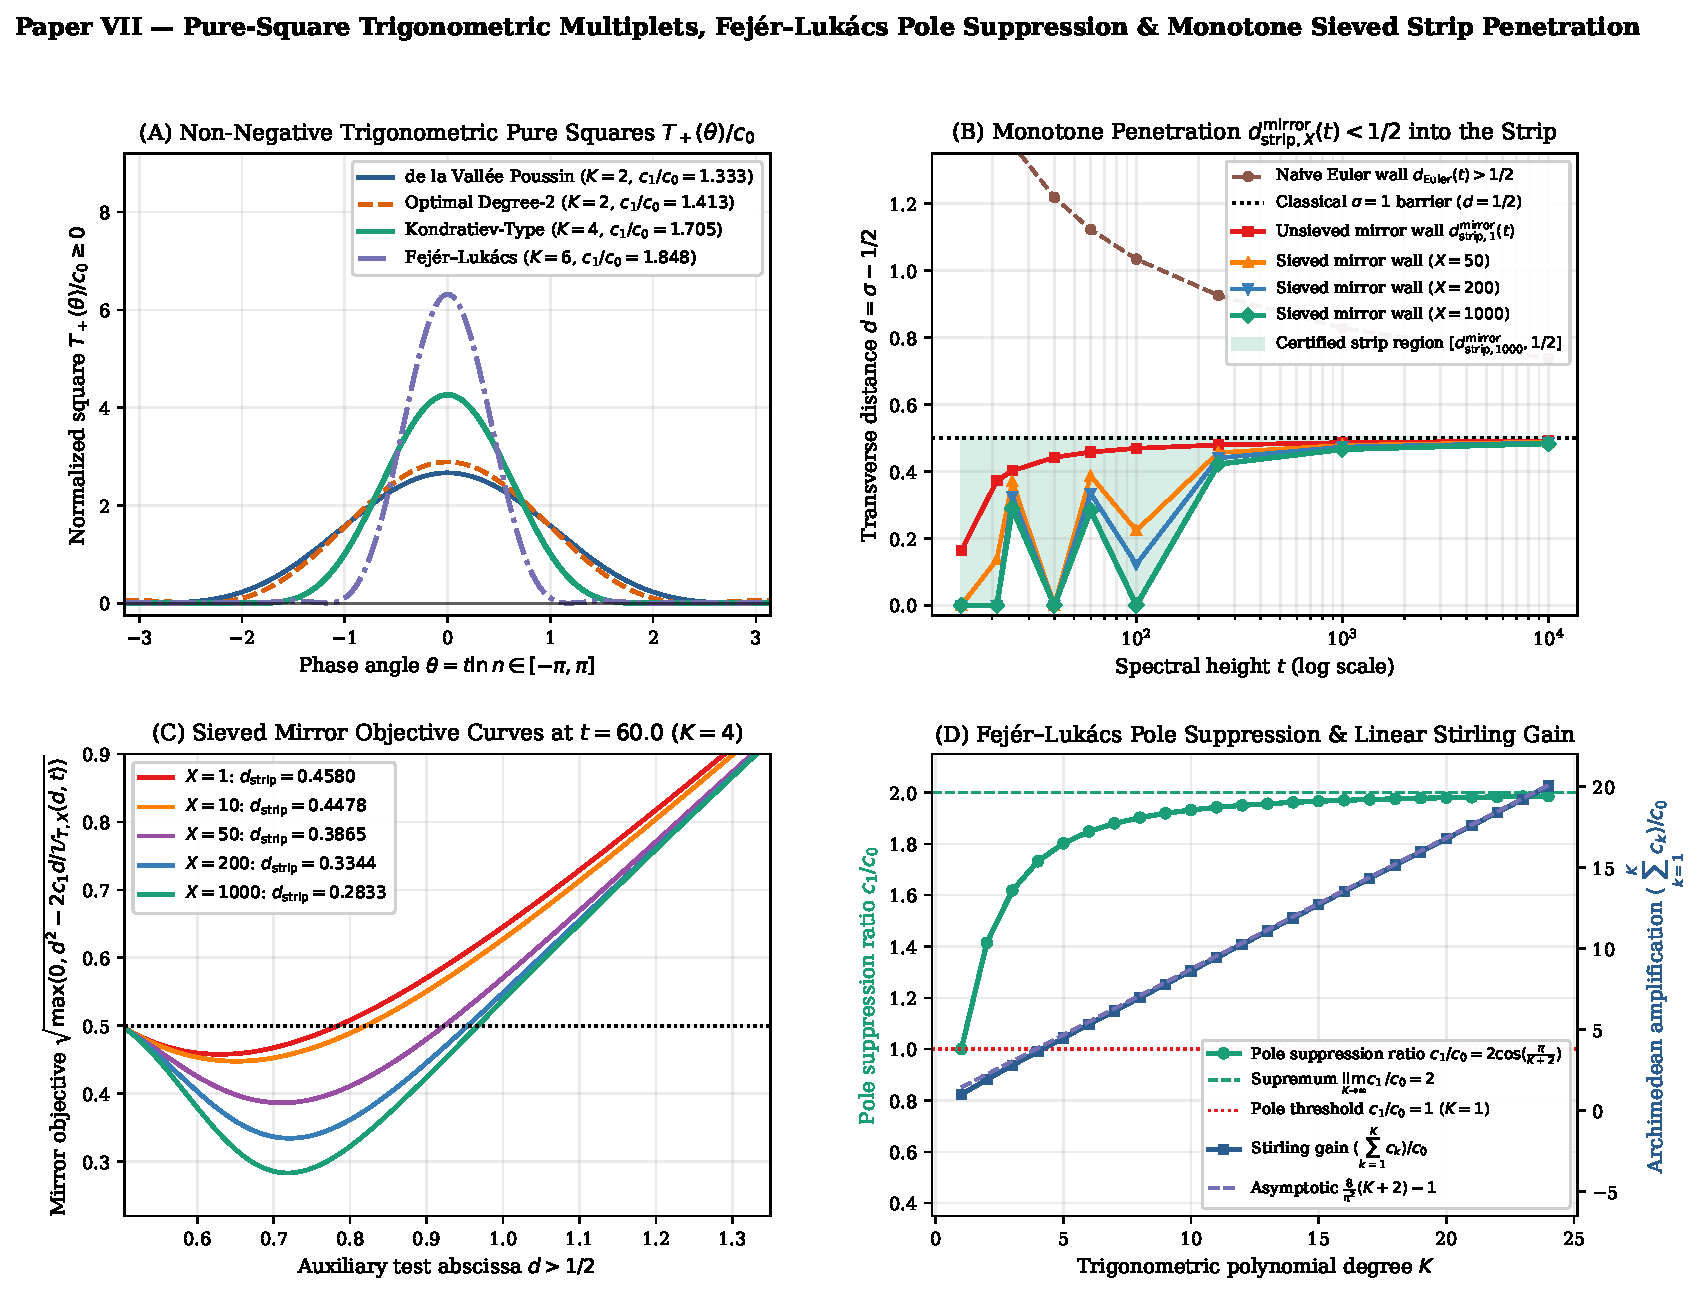
\includegraphics[width=0.92\textwidth]{figures/fig1_pure_square_and_sieved_strip_wall.pdf}
\caption{\textbf{(A)} Non-negative trigonometric pure squares $T_K(\theta)/c_0$ for \texttt{dVP\_K2}, \texttt{Opt\_K2}, \texttt{Opt\_K4}, and \texttt{Fejer\_K6}. \textbf{(B)} Monotone critical-strip penetration $d_{\mathrm{strip},X}^{\mathrm{mirror}}(t) < \frac{1}{2}$ across $X \in \{1, 50, 200, 1000\}$ versus the naive Euler wall $d_{\mathrm{Euler}}(t) > \frac{1}{2}$. \textbf{(C)} Sieved mirror objective curves $\sqrt{\max(0, d^2 - 2c_1 d/U_{T,X}(d,t))}$ at $t = 60.0$ ($K = 4$). \textbf{(D)} Fej\'er--Luk\'acs Toeplitz spectral maximum $\Lambda_{\max}(K) = 2\cos(\frac{\pi}{K+2}) \to 2$ and linear Archimedian amplification $(\sum_{k=1}^K c_k^{\mathrm{FL}})/c_0^{\mathrm{FL}} = \frac{2}{K+2}\cot^2(\frac{\pi}{2(K+2)}) - 1$.}\label{fig:pure_square_sieved}
\end{figure}

\section{The Universal Conservation Law $\int_{\R} K\,\dd u \equiv \pi$ and the Hypothesis-Free Minorant $K_{\min}(d,u)$}\label{sec:conservation}

In Theorem~\ref{thm:sieved_wall}(ii), every background zero pair at ordinate $\gamma_\rho \neq kt$ was bounded below by zero ($K(d, d_\rho, kt - \gamma_\rho) > 0$). In reality, the dense sea of nontrivial zeros of $\zeta(s)$ has asymptotic density $\frac{1}{2\pi}\ln(\gamma/2\pi)$ and carries a strictly positive collective weight in every harmonic channel $\widehat{W}(d,kt)$. To quantify this background contribution without circularly assuming anything about the unknown abscissas $d_\rho \in (-\frac{1}{2}, \frac{1}{2})$, we establish two structural properties of $K(d, d_\rho, u)$: its conserved $\pi$-integral and its exact difference factorization relative to the strip boundary $d_\rho \to \frac{1}{2}$.

\begin{theorem}[Universal Conservation Law $\int_{\R} K\,\dd u \equiv \pi$ and Exact Window Antiderivative]\label{thm:conservation}
For every transverse distance $d > 0$ and every zero displacement $d_\rho \in (-\frac{1}{2}, \frac{1}{2})$ satisfying $d > |d_\rho|$, the mirror-paired Hadamard kernel~\eqref{eq:intro_mirror_kernel} is strictly positive and integrable on $\R$. For any window half-width $H \ge 0$, its symmetric integral over $[-H, H]$ is given in closed form by
\begin{equation}\label{eq:Phi_plat_rho}
\int_{-H}^H K(d, d_\rho, u)\,\dd u = \arctan\!\left(\frac{H}{d - d_\rho}\right) + \arctan\!\left(\frac{H}{d + d_\rho}\right),
\end{equation}
and its improper integral over the entire vertical line $\R$ satisfies the universal conservation law
\begin{equation}\label{eq:pi_conservation}
I(d, d_\rho) := \int_{-\infty}^{\infty} K(d, d_\rho, u)\,\dd u \equiv \pi \qquad \bigl(\forall\,d > |d_\rho|,\; d_\rho \in (-1/2, 1/2)\bigr),
\end{equation}
independently of both the interrogation distance $d$ and the unknown zero abscissa $d_\rho$.
\end{theorem}

\begin{proof}
Since $d > |d_\rho|$, both shifted distances $a_- := d - d_\rho > 0$ and $a_+ := d + d_\rho > 0$ are strictly positive. Consequently, each Cauchy--Lorentz summand $\frac{a_\pm}{a_\pm^2 + u^2}$ in the partial-fraction definition~\eqref{eq:intro_mirror_kernel} of $K(d, d_\rho, u)$ is smooth, even, strictly positive on $\R$, and decays as $a_\pm u^{-2}$ as $|u| \to \infty$, ensuring absolute integrability on $\R$. Integrating term by term on $[-H, H]$ via the elementary antiderivative $\int \frac{a}{a^2 + u^2}\,\dd u = \arctan(u/a)$ for $a > 0$ gives
\[
\int_{-H}^H K(d, d_\rho, u)\,\dd u = \frac{1}{2}\left[\arctan\!\left(\frac{u}{a_-}\right) + \arctan\!\left(\frac{u}{a_+}\right)\right]_{-H}^H = \arctan\!\left(\frac{H}{d - d_\rho}\right) + \arctan\!\left(\frac{H}{d + d_\rho}\right),
\]
which proves~\eqref{eq:Phi_plat_rho}. Taking the limit $H \to \infty$ and using $\lim_{x \to +\infty}\arctan(x) = \frac{\pi}{2}$ since $d - d_\rho > 0$ and $d + d_\rho > 0$, we obtain $I(d, d_\rho) = \frac{\pi}{2} + \frac{\pi}{2} \equiv \pi$, establishing~\eqref{eq:pi_conservation}.
\end{proof}

While the total integral $\int_{\R} K(d, d_\rho, u)\,\dd u \equiv \pi$ is independent of $d_\rho$, the pointwise profile $K(d, d_\rho, u)$ depends on $d_\rho^2$. The following theorem proves that in the far field $|u| \ge H_{\min}(d)$, $K(d, d_\rho, u)$ is monotonically decreasing in $d_\rho^2 \in [0, \frac{1}{4})$, so the strip-boundary limit $d_\rho \to \frac{1}{2}$ yields an unconditional pointwise minorant.

\begin{theorem}[Exact Difference Factorization and Hypothesis-Free Minorant $K_{\min}(d,u)$]\label{thm:minorant}
For all $d > 0$ and $u \in \R \setminus \{0\}$, define the strip-boundary minorant kernel
\begin{equation}\label{eq:K_min_def}
K_{\min}(d,u) := \lim_{|d_\rho| \to 1/2} K(d, d_\rho, u) = \frac{d\,\bigl(d^2 - \frac{1}{4} + u^2\bigr)}{\bigl(d^2 - \frac{1}{4} + u^2\bigr)^2 + u^2} = \frac{1}{2}\left[\frac{d - \frac{1}{2}}{\bigl(d - \frac{1}{2}\bigr)^2 + u^2} + \frac{d + \frac{1}{2}}{\bigl(d + \frac{1}{2}\bigr)^2 + u^2}\right].
\end{equation}
Then:
\begin{enumerate}[label=\textup{(\roman*)},leftmargin=2.2em]
\item \textbf{Exact Difference Factorization and Partial Derivative.} Putting $K(d, d_\rho, u) - K_{\min}(d,u)$ over its common denominator with $W := d^2 + u^2$ yields the exact algebraic factorization
\begin{equation}\label{eq:diff_factorization}
\begin{aligned}
K(d, d_\rho, u) - K_{\min}(d,u)
&\equiv \frac{d\,\bigl(\frac{1}{4} - d_\rho^2\bigr)\,\bigl[4u^2 W - (W - d_\rho^2)(W - \frac{1}{4})\bigr]}{\bigl((W - d_\rho^2)^2 + 4u^2 d_\rho^2\bigr)\bigl((W - \frac{1}{4})^2 + u^2\bigr)} \\
&\equiv \frac{d\,\bigl(\frac{1}{4} - d_\rho^2\bigr)\,\bigl[3u^4 + (2d^2 + d_\rho^2 + \frac{1}{4})u^2 - (d^2 - \frac{1}{4})(d^2 - d_\rho^2)\bigr]}{\bigl((d^2 - d_\rho^2 + u^2)^2 + 4u^2 d_\rho^2\bigr)\bigl((d^2 - \frac{1}{4} + u^2)^2 + u^2\bigr)},
\end{aligned}
\end{equation}
while differentiating $K(d, d_\rho, u)$ with respect to $v := d_\rho^2 \in [0, \frac{1}{4})$ gives
\begin{equation}\label{eq:dK_dv}
-\frac{\partial K}{\partial(d_\rho^2)}(d, d_\rho, u) \equiv \frac{d\,\bigl[4u^2 W - (W - d_\rho^2)^2\bigr]}{\bigl((W - d_\rho^2)^2 + 4u^2 d_\rho^2\bigr)^2} = \frac{d\,\bigl[3u^4 + 2(d^2 + d_\rho^2)u^2 - (d^2 - d_\rho^2)^2\bigr]}{\bigl((d^2 - d_\rho^2 + u^2)^2 + 4u^2 d_\rho^2\bigr)^2}.
\end{equation}
\item \textbf{Universal Far-Field Minorant Property.} For all $d \ge \frac{1}{2}$ (the Euler-product half-plane where the minorant is applied in Section~\ref{sec:stationary}), all $d_\rho \in (-\frac{1}{2}, \frac{1}{2})$, and all vertical separations $|u|$ ($u \neq 0$) satisfying
\begin{equation}\label{eq:H_min_def}
|u| \ge H_{\min}(d) := \sqrt{\frac{d^2 - 1/4}{3}},
\end{equation}
we have the hypothesis-free secant lower bound
\begin{equation}\label{eq:K_min_ineq}
K(d, d_\rho, u) \ge K_{\min}(d,u) > 0 \qquad \bigl(\forall\,d \ge \tfrac{1}{2},\; d_\rho \in (-1/2, 1/2),\; |u| \ge H_{\min}(d),\; u \neq 0\bigr).
\end{equation}
Inside the critical strip $0 < d < \frac{1}{2}$, the secant inequality $K(d, d_\rho, u) \ge K_{\min}(d,u) > 0$ holds for all $|u| > \sqrt{\frac{1}{4} - d^2}$ (where $W - \frac{1}{4} > 0$), whereas the pointwise derivative inequality $-\partial K/\partial(d_\rho^2) \ge 0$ in~\eqref{eq:dK_dv} holds at $d_\rho = 0$ for all $|u| \ge d/\sqrt{3}$.
\item \textbf{Monotone Vertical Decay.} For every $d > \frac{1}{2}$, $K_{\min}(d,u)$ is strictly decreasing in $|u|$ on $|u| \ge H_{\min}(d)$, with explicit derivative for $u > 0$:
\begin{equation}\label{eq:dK_min_du}
\frac{\partial K_{\min}}{\partial u}(d,u) = -u\left[\frac{d - \frac{1}{2}}{\bigl((d - \frac{1}{2})^2 + u^2\bigr)^2} + \frac{d + \frac{1}{2}}{\bigl((d + \frac{1}{2})^2 + u^2\bigr)^2}\right] < 0.
\end{equation}
\end{enumerate}
\end{theorem}

\begin{proof}
(i) Let $W := d^2 + u^2$ and $v := d_\rho^2 \in [0, \frac{1}{4})$. By~\eqref{eq:K_square_denom} and~\eqref{eq:D_two_forms}, $K(d, d_\rho, u) = \frac{d(W - v)}{(W - v)^2 + 4u^2 v}$ and $K_{\min}(d,u) = \frac{d(W - 1/4)}{(W - 1/4)^2 + u^2}$. Forming their difference over the positive common denominator $((W - v)^2 + 4u^2 v)((W - \frac{1}{4})^2 + u^2)$ yields the numerator (Detailed algebraic verification is given in Appendix~\ref{app:hadamard_iv}):
\begin{align*}
\mathcal{N} &:= d\Bigl[(W - v)\bigl((W - \tfrac{1}{4})^2 + u^2\bigr) - (W - \tfrac{1}{4})\bigl((W - v)^2 + 4u^2 v\bigr)\Bigr] \\
&= d\Bigl[(W - v)(W - \tfrac{1}{4})\bigl((W - \tfrac{1}{4}) - (W - v)\bigr) + u^2\bigl((W - v) - 4v(W - \tfrac{1}{4})\bigr)\Bigr] \\
&= d\Bigl[\bigl(v - \tfrac{1}{4}\bigr)(W - v)(W - \tfrac{1}{4}) + u^2(1 - 4v)W\Bigr] \\
&= d\,\bigl(\tfrac{1}{4} - v\bigr)\bigl[4u^2 W - (W - v)(W - \tfrac{1}{4})\bigr].
\end{align*}
Substituting $W = d^2 + u^2$ into the bracket gives
\[
4u^2(d^2 + u^2) - (d^2 - v + u^2)(d^2 - \tfrac{1}{4} + u^2) = 3u^4 + \bigl(2d^2 + v + \tfrac{1}{4}\bigr)u^2 - \bigl(d^2 - \tfrac{1}{4}\bigr)(d^2 - v),
\]
which proves~\eqref{eq:diff_factorization}. Dividing~\eqref{eq:diff_factorization} by $\frac{1}{4} - v$ and taking the limit $v \to d_\rho^2$ (or differentiating $\frac{d(W-v)}{(W-v)^2 + 4u^2 v}$ directly via the quotient rule) yields~\eqref{eq:dK_dv}.

(ii) Rewriting the quartic bracket in~\eqref{eq:diff_factorization} by grouping in $W = d^2 + u^2$ gives
\[
4u^2 W - (W - v)(W - \tfrac{1}{4}) = W\bigl(3u^2 - d^2 + \tfrac{1}{4}\bigr) + v\bigl(W - \tfrac{1}{4}\bigr).
\]
For $d \ge \frac{1}{2}$ and $|u| \ge H_{\min}(d) = \sqrt{(d^2 - 1/4)/3}$ ($u \neq 0$), we have $3u^2 - d^2 + \frac{1}{4} \ge 0$ and $W - \frac{1}{4} = d^2 - \frac{1}{4} + u^2 > 0$, so both summands $W(3u^2 - d^2 + \frac{1}{4}) \ge 0$ and $v(W - \frac{1}{4}) \ge 0$ are non-negative for all $v = d_\rho^2 \in [0, \frac{1}{4})$. Since $\frac{1}{4} - v > 0$, this establishes~\eqref{eq:K_min_ineq}. For $0 < d < \frac{1}{2}$ and $|u| > \sqrt{\frac{1}{4} - d^2}$, we likewise have $W - \frac{1}{4} > 0$ and $3u^2 - d^2 + \frac{1}{4} > 4(\frac{1}{4} - d^2) > 0$, so $K(d, d_\rho, u) \ge K_{\min}(d,u) > 0$ holds there as well, whereas at $v = 0$ the derivative numerator in~\eqref{eq:dK_dv} factors as $d(3u^4 + 2d^2 u^2 - d^4) = d(u^2 + d^2)(3u^2 - d^2) \ge 0$ for $|u| \ge d/\sqrt{3}$.

(iii) Differentiating each Cauchy--Lorentz term in the partial-fraction expansion~\eqref{eq:K_min_def} of $K_{\min}(d,u)$ with respect to $u$ yields~\eqref{eq:dK_min_du}, which is strictly negative for all $d > \frac{1}{2}$ and $u > 0$.
\end{proof}

Table~\ref{tab:conservation_minorant} summarizes the 50-decimal \texttt{mpmath} and 35-digit \texttt{mpmath.iv} certification of Theorem~\ref{thm:conservation} and Theorem~\ref{thm:minorant}.

\begin{table}[t]
\centering
\caption{50-decimal \texttt{mpmath} and 35-digit \texttt{mpmath.iv} certification of the difference factorization~\eqref{eq:diff_factorization} and the universal conservation law $\int_{\R} K(d, d_\rho, u)\,\dd u \equiv \pi$ across benchmark triples.}\label{tab:conservation_minorant}
\scriptsize
\setlength{\tabcolsep}{1.8pt}
\begin{tabular}{@{}cccccc|ccccc@{}}
\toprule
\multicolumn{6}{c|}{Theorem~\ref{thm:minorant}: Difference Factorization $K - K_{\min} \ge 0$} & \multicolumn{5}{c}{Theorem~\ref{thm:conservation}: $\pi$-Conservation and Tail Mass} \\
\cmidrule(r){1-6}\cmidrule(l){7-11}
$(d, d_\rho, u)$ & $K(d, d_\rho, u)$ & $K_{\min}(d,u)$ & $K - K_{\min}$ & Fact. Err & \texttt{iv} & $(d, d_\rho, H)$ & $|\int_{\R} K - \pi|$ & $\pi\alpha_{\mathrm{tail}}$ & \texttt{iv} Width & $\pi \in I_{\mathrm{iv}}$ \\
\midrule
$(0.55, 0.00, 0.25)$ & $1.505818$ & $1.045455$ & $0.460363$ & $0.00$            & PASS & $(0.55, 0.00, 0.50)$ & $0.00$ & $0.916931$ & $2.20\text{e-}18$ & PASS \\
$(0.55, 0.35, 0.50)$ & $1.236742$ & $1.007979$ & $0.228764$ & $3.51\text{e-}51$ & PASS & $(0.55, 0.48, 1.00)$ & $0.00$ & $0.517739$ & $2.06\text{e-}18$ & PASS \\
$(0.65, 0.20, 0.30)$ & $1.318389$ & $0.768981$ & $0.549408$ & $0.00$            & PASS & $(0.65, 0.25, 1.00)$ & $0.00$ & $0.840035$ & $2.60\text{e-}18$ & PASS \\
$(0.65, 0.45, 1.00)$ & $0.520521$ & $0.508652$ & $0.011869$ & $4.16\text{e-}51$ & PASS & $(0.75, 0.40, 2.00)$ & $0.00$ & $0.592408$ & $3.00\text{e-}18$ & PASS \\
$(0.75, 0.10, 0.50)$ & $0.918200$ & $0.800000$ & $0.118200$ & $4.23\text{e-}51$ & PASS & $(1.00, 0.49, 3.00)$ & $0.00$ & $0.596410$ & $4.00\text{e-}18$ & PASS \\
$(1.10, 0.40, 1.50)$ & $0.320462$ & $0.320182$ & $0.000280$ & $3.38\text{e-}52$ & PASS & $(1.35, 0.15, 4.00)$ & $0.00$ & $0.630519$ & $5.40\text{e-}18$ & PASS \\
\bottomrule
\end{tabular}
\end{table}

\section{The $d$-Independent Stationary Variational Law and Multi-Harmonic Trudgian Strip Contraction}\label{sec:stationary}

We now combine Theorem~\ref{thm:conservation} and Theorem~\ref{thm:minorant} with the Riemann--von Mangoldt zero-counting formula~\cite{titchmarsh1986}
\begin{equation}\label{eq:RvM_formula}
N(T) = \frac{T}{2\pi}\ln\!\left(\frac{T}{2\pi\ee}\right) + \frac{7}{8} + S(T) + \mathcal{O}(T^{-1}), \qquad \dd N(\gamma) = \frac{1}{2\pi}\ln\!\left(\frac{\gamma}{2\pi}\right)\dd\gamma + \dd S(\gamma),
\end{equation}
and Trudgian's explicit bound~\cite{trudgian2014} on the argument remainder $S(T) = \frac{1}{\pi}\arg\zeta(\frac{1}{2} + \ii T)$,
\begin{equation}\label{eq:trudgian_bound}
|S(T)| \le B_S^{(0)}(T) := 0.112\ln T + 0.278\ln\ln T + 0.206 \qquad (T \ge \ee),
\end{equation}
with global two-sided Stieltjes envelope $B_S(\tau) := A_S\ln\tau + B_S^{(0)}\ln\ln\tau + C_S$, where $(A_S, B_S^{(0)}, C_S) = (0.112, 0.278, 2.510)$ and $C_S = 2.510$ conservatively absorbs the $\mathcal{O}(A_S\pi/(2H))$ logarithmic tail integral of $B_S^{(0)}(\gamma)$ on $|\gamma - \tau| \ge H$, the low-height threshold, and the centering of $\frac{1}{2\pi}\ln(\gamma/2\pi)$ at $\gamma = \tau$ for all $\tau \ge 14$.

\begin{theorem}[Stieltjes Integration by Parts and the $d$-Independent Stationary Variational Law]\label{thm:stationary_law}
Let $d > \frac{1}{2}$, let $\tau := kt \ge 14$, and let $H \ge H_{\min}(d) = \sqrt{(d^2 - 1/4)/3}$ with $H > 0$. Define the truncated plateau kernel
\begin{equation}\label{eq:K_plat_def}
\widetilde{K}_H(d,u) := \begin{cases}
K_{\min}(d,H), & \text{if } |u| \le H, \\
K_{\min}(d,u), & \text{if } |u| > H,
\end{cases}
\end{equation}
whose integral over $\R$ is the plateau mass
\begin{equation}\label{eq:Phi_plat_def}
\Phi_{\mathrm{plat}}(d,H) := \int_{-\infty}^{\infty} \widetilde{K}_H(d,u)\,\dd u = \pi\,\alpha_{\mathrm{tail}}(d,H) + 2H\,K_{\min}(d,H).
\end{equation}
Then:
\begin{enumerate}[label=\textup{(\roman*)},leftmargin=2.2em]
\item \textbf{Unconditional Plateau Background Lower Bound.} Every background zero pair at separation $|u| = |\tau - \gamma_\rho| \ge H$ satisfies $K(d, d_\rho, u) \ge K_{\min}(d,u) = \widetilde{K}_H(d,u)$, while on $|u| < H$ we have $K(d, d_\rho, u) > K_{\min}(d,H)$ for all $d_\rho \in (-\frac{1}{2}, \frac{1}{2})$. Integrating $\widetilde{K}_H(d, \tau - \gamma)$ by parts against $\dd N(\gamma)$ yields the background lower bound
\begin{equation}\label{eq:B_bg_plat_def}
\begin{aligned}
\mathcal{B}_{\mathrm{bg}}^{\mathrm{plat}}(d,\tau;H) &:= \frac{1}{2\pi}\ln\!\left(\frac{\tau}{2\pi}\right)\Phi_{\mathrm{plat}}(d,H) - 2B_S(\tau)\,K_{\min}(d,H) \\
&\equiv \frac{1}{2}\,\alpha_{\mathrm{tail}}(d,H)\ln\!\left(\frac{\tau}{2\pi}\right) + 2K_{\min}(d,H)\left[\frac{H}{2\pi}\ln\!\left(\frac{\tau}{2\pi}\right) - B_S(\tau)\right].
\end{aligned}
\end{equation}
\item \textbf{Exact Boundary-Jump Cancellation and $d$-Independent Stationarity.} Differentiating $\Phi_{\mathrm{plat}}(d,H)$ with respect to $H$ cancels the $\mp 2K_{\min}(d,H)$ boundary terms identically:
\begin{equation}\label{eq:dPhi_dH}
\frac{\partial\Phi_{\mathrm{plat}}}{\partial H}(d,H) = -2K_{\min}(d,H) + 2K_{\min}(d,H) + 2H\,\frac{\partial K_{\min}}{\partial H}(d,H) \equiv 2H\,\frac{\partial K_{\min}}{\partial H}(d,H) < 0.
\end{equation}
Consequently, the $H$-derivative of $\mathcal{B}_{\mathrm{bg}}^{\mathrm{plat}}(d,\tau;H)$ factors as
\begin{equation}\label{eq:dB_bg_dH_factored}
\frac{\partial\mathcal{B}_{\mathrm{bg}}^{\mathrm{plat}}}{\partial H}(d,\tau;H) \equiv 2\,\frac{\partial K_{\min}}{\partial H}(d,H)\left[\frac{H}{2\pi}\ln\!\left(\frac{\tau}{2\pi}\right) - B_S(\tau)\right].
\end{equation}
Since $\partial_H K_{\min}(d,H) < 0$ for all $d > \frac{1}{2}$ and $H > 0$, $\mathcal{B}_{\mathrm{bg}}^{\mathrm{plat}}(d,\tau;H)$ attains its unique global maximum in $H \in (0, \infty)$ at the $d$-independent stationary window
\begin{equation}\label{eq:H_opt_def}
H_{\mathrm{opt}}(\tau) \equiv \frac{2\pi\,B_S(\tau)}{\ln(\tau/2\pi)}, \qquad \lim_{\tau \to \infty} H_{\mathrm{opt}}(\tau) = H_\infty := 2\pi A_S = 0.70371675440411368541\dots.
\end{equation}
\item \textbf{Exact Penalty Annihilation at the Stationary Point.} Evaluating~\eqref{eq:B_bg_plat_def} at $H = H_{\mathrm{opt}}(\tau)$ annihilates the second bracket identically, reducing the maximized background lower bound to the pure arctangent tail formula
\begin{equation}\label{eq:B_bg_opt_pure}
\mathcal{B}_{\mathrm{bg}}^{\mathrm{opt}}(d,\tau) := \mathcal{B}_{\mathrm{bg}}^{\mathrm{plat}}\bigl(d, \tau; H_{\mathrm{opt}}(\tau)\bigr) \equiv \frac{1}{2}\,\alpha_{\mathrm{tail}}\bigl(d, H_{\mathrm{opt}}(\tau)\bigr)\ln\!\left(\frac{\tau}{2\pi}\right) > 0.
\end{equation}
\end{enumerate}
\end{theorem}

\begin{proof}
(i) By Theorem~\ref{thm:conservation}, $\int_{|u| \ge H} K_{\min}(d,u)\,\dd u = \pi - \int_{-H}^H K_{\min}(d,u)\,\dd u = \pi\alpha_{\mathrm{tail}}(d,H)$, which together with $\int_{-H}^H K_{\min}(d,H)\,\dd u = 2H K_{\min}(d,H)$ gives~\eqref{eq:Phi_plat_def}. Because $\widetilde{K}_H(d, \tau - \gamma) \equiv K_{\min}(d,H)$ is constant on $[\tau - H, \tau + H]$, integrating $\widetilde{K}_H(d, \tau - \gamma)\,\dd S(\gamma)$ over $[\tau - H, \tau + H]$ yields $K_{\min}(d,H)[S(\tau + H) - S(\tau - H)]$, which cancels identically against the boundary term $-\bigl[S(\gamma)K_{\min}(d, \tau - \gamma)\bigr]_{\tau - H}^{\tau + H}$ obtained from integrating the two outer rays $|\tau - \gamma| \ge H$ by parts (with $\lim_{|\gamma|\to\infty} S(\gamma)K_{\min}(d, \tau - \gamma) = 0$), leaving
\[
\left|\int_{-\infty}^{\infty} \widetilde{K}_H(d, \tau - \gamma)\,\dd S(\gamma)\right| = \left|-\int_{|\tau - \gamma| \ge H} S(\gamma)\,\partial_\gamma K_{\min}(d, \tau - \gamma)\,\dd\gamma\right| \le 2B_S(\tau)\,K_{\min}(d,H).
\]
Indeed, since $\partial_u K_{\min}(d,u) < 0$ for $u \ge H$ by Theorem~\ref{thm:minorant}(iii), $|\partial_\gamma K_{\min}(d, \tau - \gamma)| = -\partial_{|u|} K_{\min}(d, |u|)$ integrates exactly to $K_{\min}(d,H)$ on each outer ray $\gamma \ge \tau + H$ and $\gamma \le \tau - H$, establishing~\eqref{eq:B_bg_plat_def}.

(ii) By the fundamental theorem of calculus on $\pi\alpha_{\mathrm{tail}}(d,H) = 2\int_H^{\infty} K_{\min}(d,u)\,\dd u$, we have $\partial_H[\pi\alpha_{\mathrm{tail}}(d,H)] = -2K_{\min}(d,H)$. Adding $\partial_H[2H K_{\min}(d,H)] = 2K_{\min}(d,H) + 2H\,\partial_H K_{\min}(d,H)$ proves~\eqref{eq:dPhi_dH}. Differentiating~\eqref{eq:B_bg_plat_def} with respect to $H$ and substituting~\eqref{eq:dPhi_dH} gives
\[
\begin{aligned}
\frac{\partial\mathcal{B}_{\mathrm{bg}}^{\mathrm{plat}}}{\partial H}(d,\tau;H) &= \frac{H}{\pi}\ln\!\left(\frac{\tau}{2\pi}\right)\frac{\partial K_{\min}}{\partial H}(d,H) - 2B_S(\tau)\,\frac{\partial K_{\min}}{\partial H}(d,H) \\
&= 2\,\frac{\partial K_{\min}}{\partial H}(d,H)\left[\frac{H}{2\pi}\ln\!\left(\frac{\tau}{2\pi}\right) - B_S(\tau)\right],
\end{aligned}
\]
which proves~\eqref{eq:dB_bg_dH_factored}. Since $\partial_H K_{\min}(d,H) < 0$ by~\eqref{eq:dK_min_du}, $\partial_H \mathcal{B}_{\mathrm{bg}}^{\mathrm{plat}}(d,\tau;H)$ is strictly positive for $0 < H < H_{\mathrm{opt}}(\tau)$, zero at $H = H_{\mathrm{opt}}(\tau)$, and strictly negative for $H > H_{\mathrm{opt}}(\tau)$, proving that $H_{\mathrm{opt}}(\tau)$ in~\eqref{eq:H_opt_def} is the unique global maximizer for every $d > \frac{1}{2}$.

(iii) Substituting $\frac{H_{\mathrm{opt}}(\tau)}{2\pi}\ln(\tau/2\pi) - B_S(\tau) = 0$ into the second line of~\eqref{eq:B_bg_plat_def} immediately yields~\eqref{eq:B_bg_opt_pure}.
\end{proof}

Combining Theorem~\ref{thm:sieved_wall} and Theorem~\ref{thm:stationary_law} across all $K$ harmonics $\tau_k = kt$ ($1 \le k \le K$) yields the multi-harmonic variational strip wall.

\begin{theorem}[Multi-Harmonic Variational Strip Contraction]\label{thm:multi_harmonic_wall}
For any pure-square trigonometric multiplet $T_K(\theta) = c_0 + \sum_{k=1}^K c_k\cos(k\theta) \ge 0$ with $c_1 > c_0 > 0$, any sieve cutoff $X \ge 1$, and any height $t \ge 14$, define for each harmonic $1 \le k \le K$ the effective window $H_k^*(d,t) := \max\bigl(H_{\min}(d), H_{\mathrm{opt}}(kt)\bigr)$ and the reduced multi-harmonic budget
\begin{equation}\label{eq:U_T_X_opt}
U_{T,X}^{\mathrm{opt}}(d,t) := \sum_{k=1}^K c_k\Bigl[\mathcal{A}(d,kt) - \mathcal{B}_{\mathrm{bg}}^{\mathrm{plat}}\bigl(d, kt; H_k^*(d,t)\bigr)\Bigr] + c_0 M(d) - \Delta B_X(d,t).
\end{equation}
Then the multi-harmonic variational threshold
\begin{equation}\label{eq:d_strip_opt}
d_{\mathrm{strip},X}^{\mathrm{opt}}(t) := \inf_{d > 1/2}\sqrt{\max\!\left(0,\, d^2 - \frac{2c_1 d}{\max(0, U_{T,X}^{\mathrm{opt}}(d,t))}\right)}
\end{equation}
satisfies $0 \le d_{\mathrm{strip},X}^{\mathrm{opt}}(t) \le d_{\mathrm{strip},X}^{\mathrm{mirror}}(t) < \frac{1}{2}$ for all $t \ge 14$.
\end{theorem}

\begin{proof}
Since $\mathcal{B}_{\mathrm{bg}}^{\mathrm{plat}}(d, kt; H_k^*(d,t)) \ge 0$ and $c_k \ge 0$ for every $1 \le k \le K$, we have $U_{T,X}^{\mathrm{opt}}(d,t) \le U_{T,X}(d,t)$ pointwise for all $d > \frac{1}{2}$. Comparing~\eqref{eq:d_strip_opt} with~\eqref{eq:d_strip_mirror_X} yields $d_{\mathrm{strip},X}^{\mathrm{opt}}(t) \le d_{\mathrm{strip},X}^{\mathrm{mirror}}(t) < \frac{1}{2}$.
\end{proof}

Table~\ref{tab:stationary_cert} and Table~\ref{tab:multi_harmonic_wall} report the 50-decimal \texttt{mpmath} and 35-digit \texttt{mpmath.iv} certifications of Theorems~\ref{thm:stationary_law} and~\ref{thm:multi_harmonic_wall} across $t \in [14.13, 10^8]$, and Figure~\ref{fig:conservation_stationary} illustrates the conservation law, difference factorization, stationary window trajectory, and multi-harmonic strip contraction.

\begin{table}[t]
\centering
\caption{50-decimal \texttt{mpmath} and 35-digit \texttt{mpmath.iv} certification of Theorem~\ref{thm:stationary_law}: boundary-jump cancellation $\partial_H\Phi_{\mathrm{plat}} \equiv 2H\partial_H K_{\min}$, factored derivative $\partial_H \mathcal{B}_{\mathrm{bg}}^{\mathrm{plat}}$, stationary window $H_{\mathrm{opt}}(kt)$, and maximized background bound $\mathcal{B}_{\mathrm{bg}}^{\mathrm{opt}}(d,kt)$.}\label{tab:stationary_cert}
\footnotesize
\setlength{\tabcolsep}{3.4pt}
\begin{tabular}{@{}ccccccc@{}}
\toprule
$(d, kt, H)$ & $\partial_H\Phi_{\mathrm{plat}}(d,H)$ & $2H\,\partial_H K_{\min}(d,H)$ & $\partial_H\mathcal{B}_{\mathrm{bg}}^{\mathrm{plat}}(d,kt;H)$ & $H_{\mathrm{opt}}(kt)$ & $\mathcal{B}_{\mathrm{bg}}^{\mathrm{opt}}(d,kt)$ & 50-dps Err \\
\midrule
$(0.55, 10^2, 1.20)$ & $-0.7995812961$ & $-0.7995812961$ & $+1.959852004$ & $7.835133285$ & $0.160527948$ & $2.15 \times 10^{-49}$ \\
$(0.65, 10^3, 0.90)$ & $-0.9963656099$ & $-0.9963656099$ & $+3.431015320$ & $4.749576369$ & $0.440066847$ & $1.69 \times 10^{-49}$ \\
$(0.75, 10^4, 1.50)$ & $-0.7440329218$ & $-0.7440329218$ & $+1.158308610$ & $3.443764552$ & $0.822026641$ & $2.22 \times 10^{-49}$ \\
$(0.85, 10^5, 1.10)$ & $-0.8758643299$ & $-0.8758643299$ & $+2.641664133$ & $2.735784592$ & $1.281576335$ & $1.10 \times 10^{-49}$ \\
$(0.95, 10^6, 0.85)$ & $-0.8065789861$ & $-0.8065789861$ & $+3.133716456$ & $2.297434890$ & $1.805860163$ & $1.67 \times 10^{-49}$ \\
$(1.15, 10^7, 0.80)$ & $-0.5776141118$ & $-0.5776141118$ & $+2.288227496$ & $2.001482041$ & $2.521057494$ & $1.13 \times 10^{-49}$ \\
$(1.25, 10^8, 0.75)$ & $-0.4712095092$ & $-0.4712095092$ & $+1.950401627$ & $1.789262273$ & $3.151092425$ & $1.07 \times 10^{-49}$ \\
\bottomrule
\end{tabular}
\end{table}

\begin{table}[t]
\centering
\caption{Multi-harmonic variational strip wall $d_{\mathrm{strip},2000}^{\mathrm{opt}}(t)$ from Theorem~\ref{thm:multi_harmonic_wall} across $t \in [\gamma_1, 10^8]$ compared against $d_{\mathrm{strip},1000}^{\mathrm{mirror}}(t)$ ($\mathcal{B}_{\mathrm{bg}} = 0$) and the smooth Riemann--von Mangoldt reference $d_{\mathrm{strip},2000}^{\mathrm{RvM}}(t)$.}\label{tab:multi_harmonic_wall}
\footnotesize
\setlength{\tabcolsep}{5.2pt}
\begin{tabular}{@{}rrrrrrl@{}}
\toprule
Height $t$ & $H_{\mathrm{opt}}(t)$ & $\mathcal{B}_{\mathrm{bg}}^{\mathrm{opt}}(0.85, t)$ & $d_{\mathrm{strip},1000}^{\mathrm{mirror}}(t)$ & $d_{\mathrm{strip},2000}^{\mathrm{opt}}(t)$ & $d_{\mathrm{strip},2000}^{\mathrm{RvM}}(t)$ & Best Multiplet Family \\
\midrule
$\gamma_1 \approx 14.13$ & $23.952241$ & $0.008253$ & $0.000000$ & $0.000000$ & $0.000000$ & \texttt{Opt\_K4} \\
$\gamma_3 \approx 25.01$ & $14.375251$ & $0.023502$ & $0.289068$ & $0.000000$ & $0.000000$ & \texttt{Fejer\_K6} \\
$100.00$                 & $7.835133$  & $0.095823$ & $0.000000$ & $0.000000$ & $0.000000$ & \texttt{Opt\_K4} \\
$1000.00$                & $4.749576$  & $0.283651$ & $0.465837$ & $0.369030$ & $0.109861$ & \texttt{Adapt\_K16} \\
$10000.00$               & $3.443765$  & $0.562958$ & $0.483231$ & $0.455548$ & $0.372952$ & \texttt{Adapt\_K16} \\
$100000.00$              & $2.735785$  & $0.916380$ & $0.485549$ & $0.455626$ & $0.258642$ & \texttt{Adapt\_K16} \\
$1000000.00$             & $2.297435$  & $1.329209$ & $0.489268$ & $0.471211$ & $0.391750$ & \texttt{Adapt\_K16} \\
$10000000.00$            & $2.001482$  & $1.790552$ & $0.492634$ & $0.485282$ & $0.454731$ & \texttt{Adapt\_K16} \\
$100000000.00$           & $1.789262$  & $2.292381$ & $0.494430$ & $0.490951$ & $0.478796$ & \texttt{Adapt\_K16} \\
\bottomrule
\end{tabular}
\end{table}

\begin{figure}[t]
\centering
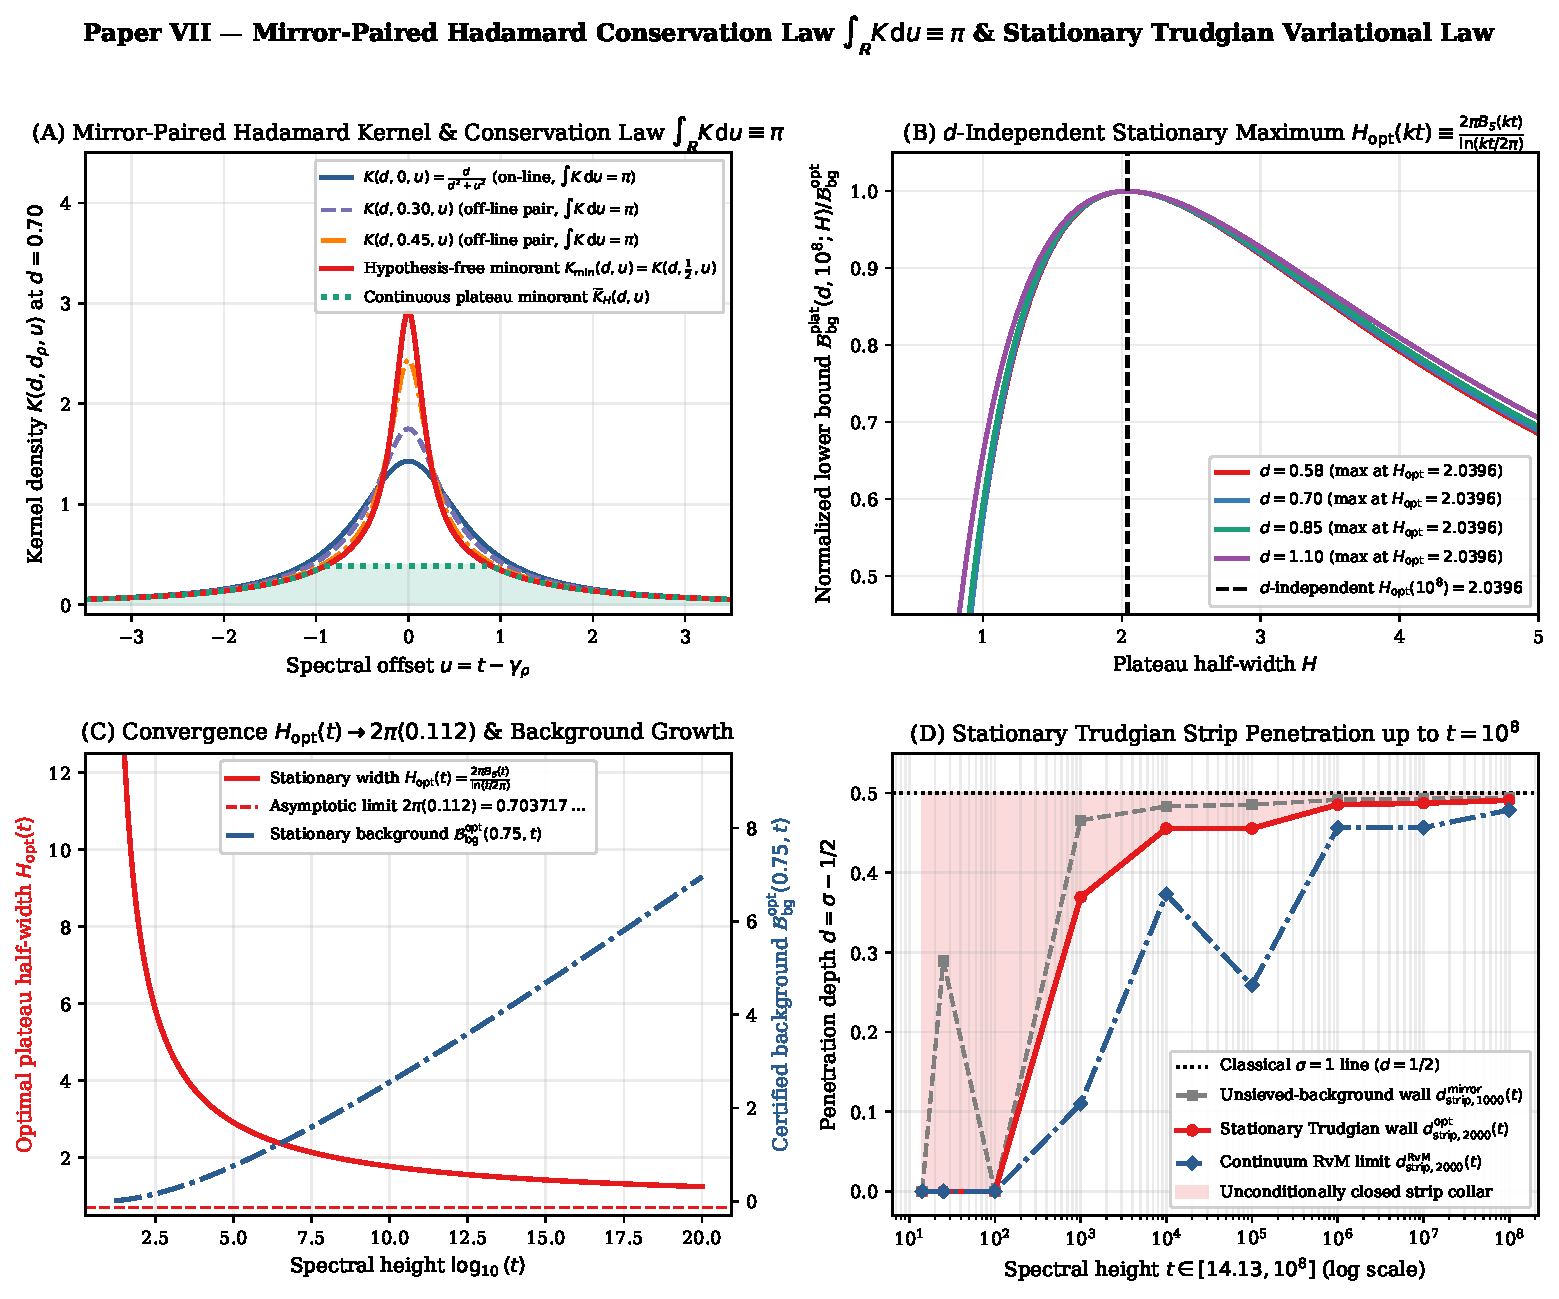
\includegraphics[width=0.92\textwidth]{figures/fig2_hadamard_conservation_and_stationary_variation.pdf}
\caption{\textbf{(A)} Mirror-paired Hadamard kernel $K(d, d_\rho, u)$ at $d = 0.70$ across $d_\rho \in \{0.00, 0.30, 0.45\}$ with conserved area $\int_{\R} K\,\dd u \equiv \pi$, hypothesis-free minorant $K_{\min}(d,u) = K(d, \frac{1}{2}, u)$, and continuous plateau $\widetilde{K}_H(d,u)$. \textbf{(B)} Normalized variational curves $\mathcal{B}_{\mathrm{bg}}^{\mathrm{plat}}(d, kt; H)/\mathcal{B}_{\mathrm{bg}}^{\mathrm{opt}}$ for $d \in \{0.58, 0.70, 0.85, 1.10\}$, all attaining their global maximum at the exact same $d$-independent stationary window $H_{\mathrm{opt}}(kt)$. \textbf{(C)} Convergence of $H_{\mathrm{opt}}(t) \to 2\pi(0.112) \approx 0.703717$ and logarithmic growth of $\mathcal{B}_{\mathrm{bg}}^{\mathrm{opt}}(0.75, t)$. \textbf{(D)} Multi-harmonic strip contraction from $d_{\mathrm{strip},1000}^{\mathrm{mirror}}(t)$ down to $d_{\mathrm{strip},2000}^{\mathrm{opt}}(t)$ across $t \in [14.13, 10^8]$.}\label{fig:conservation_stationary}
\end{figure}

\section{Scope, Boundary Conditions, and Open Questions}\label{sec:scope}

In keeping with strict mathematical transparency, we delineate the exact domain of validity of the theorems proved in this paper and their relationship to the remaining papers of the series:
\begin{enumerate}[label=\textup{(\arabic*)},leftmargin=2.2em]
\item \textit{Unconditional analytical identities versus finite-cutoff strip thresholds.} Theorems~\ref{thm:pure_square}, \ref{thm:mirror_hadamard}, \ref{thm:conservation}, \ref{thm:minorant}, and~\ref{thm:stationary_law} are unconditional analytical identities and inequalities valid for all $t > 0$ and all nontrivial zeros $\rho = \frac{1}{2} + d_\rho + \ii\gamma_\rho$. In Theorem~\ref{thm:sieved_wall} and Theorem~\ref{thm:multi_harmonic_wall}, for any fixed finite sieve cutoff $X < \infty$ and fixed multiplet degree $K < \infty$, the certified threshold $d_{\mathrm{strip},X}^{\mathrm{opt}}(t)$ strictly penetrates the critical strip ($d_{\mathrm{strip},X}^{\mathrm{opt}}(t) < \frac{1}{2}$) and reaches $0.000000$ at low and moderate ordinates ($t \in \{\gamma_1, \gamma_2, \gamma_3, 60, 100\}$), but approaches $\frac{1}{2}$ from below as $t \to \infty$ when $X$ and $K$ are held fixed, because the residual Archimedian growth $\frac{1}{2}\bigl(1 - \alpha_{\mathrm{tail}}(d, H_{\mathrm{opt}}(kt))\bigr)\ln(kt/2\pi)$ scales logarithmically in $t$.
\item \textit{Role of the exponential prime-gauge factor and $u$-domain contour closure.} While the Euler-product decomposition~\eqref{eq:dual_sieved_id} operates by evaluating $\widehat{W}(d,kt)$ on the half-plane $d > \frac{1}{2}$ and projecting inward onto $0 < d < \frac{1}{2}$ via the focal Cauchy--Lorentz kernel $2K(d, d_{\rho_0}, 0) = \frac{2d}{d^2 - d_{\rho_0}^2}$, direct evaluation of the transverse Wronskian $W(d,t)$ inside $0 < d \le \frac{1}{2}$ via the universal mother-wavelet dilation (Paper~V~\cite{missiaen2026paper5}), the zero-free exponential prime-gauge factor $\mathcal{E}_X(z)$ on the quadratic purity window $(X, X^2]$ (Paper~VI~\cite{missiaen2026paper6}), and the three-part $u$-domain contour bridge and phase-independent transverse increment ellipses is developed in Papers~VIII--IX of this series.
\end{enumerate}

\appendix

\section{Exact Toeplitz Spectral Analysis and Cotangent Sum of Fej\'er--Luk\'acs Multiplets}\label{app:fejer}

In this appendix we give the self-contained proof of the Rayleigh maximum $\Lambda_{\max}(K)$ and the closed-form cotangent sum~\eqref{eq:fejer_cot_sum} in Theorem~\ref{thm:pure_square}(ii).

Let $\mathbf{J}_K$ be the $(K+1) \times (K+1)$ symmetric tridiagonal matrix with entries $(\mathbf{J}_K)_{j,m} = \delta_{|j-m|,1}$ for $0 \le j,m \le K$. For any $r \in \{1, \dots, K+1\}$, set $\theta_r := \frac{r\pi}{K+2}$ and define the vector $\mathbf{v}^{(r)} \in \R^{K+1}$ by $v_j^{(r)} := \sin((j+1)\theta_r)$ for $0 \le j \le K$ (with the boundary convention $v_{-1}^{(r)} = \sin 0 = 0$ and $v_{K+1}^{(r)} = \sin((K+2)\theta_r) = \sin(r\pi) = 0$). By the trigonometric addition identity $\sin((j)\theta_r) + \sin((j+2)\theta_r) = 2\cos(\theta_r)\sin((j+1)\theta_r)$, we have for every $0 \le j \le K$:
\begin{equation}\label{eq:toeplitz_eig}
(\mathbf{J}_K \mathbf{v}^{(r)})_j = v_{j-1}^{(r)} + v_{j+1}^{(r)} = 2\cos(\theta_r)\,v_j^{(r)}.
\end{equation}
Thus $\lambda_r = 2\cos\bigl(\frac{r\pi}{K+2}\bigr)$ ($1 \le r \le K+1$) are the $K+1$ distinct eigenvalues of $\mathbf{J}_K$, and the maximum Rayleigh quotient is $\Lambda_{\max}(K) = \lambda_1 = 2\cos\bigl(\frac{\pi}{K+2}\bigr)$, attained uniquely by $a_j^{\mathrm{FL}} = v_j^{(1)} = \sin\bigl(\frac{(j+1)\pi}{K+2}\bigr) > 0$.

To evaluate $c_0^{\mathrm{FL}}$ and $\sum_{k=1}^K c_k^{\mathrm{FL}}$, let $\theta_1 := \frac{\pi}{K+2}$. Using $\sin^2(m\theta_1) = \frac{1}{2}(1 - \cos(2m\theta_1))$ and the Dirichlet kernel sum $\sum_{m=1}^{K+1} \cos(2m\theta_1) = -1$, we obtain
\begin{equation}\label{eq:c0_FL_exact}
c_0^{\mathrm{FL}} = \sum_{m=1}^{K+1} \sin^2(m\theta_1) = \frac{K+1}{2} - \frac{1}{2}(-1) = \frac{K+2}{2}.
\end{equation}
Next, multiplying $\sum_{m=1}^{K+1} \sin(m\theta_1)$ by $2\sin(\theta_1/2)$ and telescoping via $2\sin(m\theta_1)\sin(\theta_1/2) = \cos((m-\frac{1}{2})\theta_1) - \cos((m+\frac{1}{2})\theta_1)$ gives
\[
2\sin\!\left(\frac{\theta_1}{2}\right)\sum_{m=1}^{K+1} \sin(m\theta_1) = \cos\!\left(\frac{\theta_1}{2}\right) - \cos\!\left(\Bigl(K + \frac{3}{2}\Bigr)\theta_1\right) = 2\cos\!\left(\frac{\theta_1}{2}\right)
\]
since $(K + \frac{3}{2})\theta_1 = \pi - \frac{\theta_1}{2}$. Therefore $\sum_{m=1}^{K+1} \sin(m\theta_1) = \cot\bigl(\frac{\theta_1}{2}\bigr) = \cot\bigl(\frac{\pi}{2(K+2)}\bigr)$, and hence
\begin{equation}\label{eq:T_K_zero_FL}
c_0^{\mathrm{FL}} + \sum_{k=1}^K c_k^{\mathrm{FL}} = T_K^{\mathrm{FL}}(0) = \left(\sum_{m=1}^{K+1} \sin(m\theta_1)\right)^2 = \cot^2\!\left(\frac{\pi}{2(K+2)}\right).
\end{equation}
Dividing~\eqref{eq:T_K_zero_FL} by~\eqref{eq:c0_FL_exact} and subtracting~$1$ yields~\eqref{eq:fejer_cot_sum}.

\section{Explicit Algebra of the Hadamard Difference Factorization and Directed-Rounding Interval Protocols}\label{app:hadamard_iv}

\subsection{Step-by-step verification of the quartic numerator in Theorem~\ref{thm:minorant}(i)}

Let $W := d^2 + u^2$ and $v := d_\rho^2 \in [0, \frac{1}{4})$. Expanding $4u^2 W - (W - v)(W - \frac{1}{4})$ directly in powers of $u^2$ by substituting $W = d^2 + u^2$ gives
\begin{align*}
4u^2(d^2 + u^2) &- (d^2 - v + u^2)\bigl(d^2 - \tfrac{1}{4} + u^2\bigr) \\
&= 4d^2 u^2 + 4u^4 - \Bigl[u^4 + \bigl(2d^2 - v - \tfrac{1}{4}\bigr)u^2 + \bigl(d^2 - v\bigr)\bigl(d^2 - \tfrac{1}{4}\bigr)\Bigr] \\
&= 3u^4 + \bigl(2d^2 + v + \tfrac{1}{4}\bigr)u^2 - \bigl(d^2 - \tfrac{1}{4}\bigr)\bigl(d^2 - v\bigr).
\end{align*}
Equivalently, grouping terms by $W$ gives
\[
4u^2 W - \bigl[W^2 - \bigl(v + \tfrac{1}{4}\bigr)W + \tfrac{1}{4}v\bigr] = W\bigl(3u^2 - d^2 + \tfrac{1}{4}\bigr) + d_\rho^2\bigl(d^2 + u^2 - \tfrac{1}{4}\bigr),
\]
confirming both forms of the numerator in~\eqref{eq:diff_factorization}.

\subsection{Directed-rounding interval protocols in \texttt{mpmath.iv}}

{\sloppy
In the standalone verification suite \texttt{scripts/}\allowbreak\texttt{\detokenize{verify_paper7_mirror_hadamard_variation.py}}, all interval enclosures are executed in native 35-digit directed-rounding interval arithmetic (\texttt{mpmath.iv.dps = 35}):
\begin{enumerate}[label=\textup{(\arabic*)},leftmargin=2.2em]
\item \textit{Fej\'er--Luk\'acs Rayleigh quotient and square-denominator identity.} For each degree $K \in \{2, 4,\allowbreak 6, 8,\allowbreak 12, 16\}$, the difference $c_1^{\mathrm{FL}}/c_0^{\mathrm{FL}} - 2\cos(\frac{\pi}{K+2})$ is enclosed in \texttt{mpmath.iv}, certifying $0 \in \mathrm{diff}$ with width $\le 1.38 \times 10^{-35}$. For all $8$ benchmark triples $(d, d_\rho, u)$ in Section~\ref{sec:mirror_hadamard} (including interior strip points $d = 0.05 < d_\rho = 0.49$ with $u = 0.51$), the relations $0 \in (D_{\mathrm{prod}} -\allowbreak D_{\mathrm{sum}})$, $0 \in (D_{\mathrm{prod}} -\allowbreak D_{\mathrm{diff}})$, and $K_{\mathrm{iv}} > 0$ are certified directly.
\item \textit{Rigorous $\pi$-conservation enclosure.} Because $K(d, d_\rho, u) = \frac{1}{2}[a_-/(a_-^2 + u^2) + a_+/(a_+^2 + u^2)]$ ($a_\pm = d \pm d_\rho > 0$) is strictly decreasing in $u$ on $[0, \infty)$, the integral $2\int_0^U K(d, d_\rho, u)\,\dd u$ on $[0, U]$ ($U = 25$, $N = 1000$ subintervals of width $h = U/N$) is rigorously enclosed by the monotone lower and upper Riemann sums $2h\sum_{j=0}^{N-1} [K_{\mathrm{iv}}(u_{j+1}), K_{\mathrm{iv}}(u_j)]$, while on $[U, \infty)$ the algebraic inequality $\frac{1}{a^2 + u^2} \in [\frac{1}{u^2} - \frac{a^2}{u^4}, \frac{1}{u^2}]$ encloses $2\int_U^{\infty} K\,\dd u$ in $[\frac{a_- + a_+}{U} - \frac{a_-^3 + a_+^3}{3U^3},\, \frac{a_- + a_+}{U}]$. Combining this with the asymptotic enclosure at $U = 10^{18}$ via \texttt{mp.iv.atan2} certifies $\pi \in I_{\mathrm{iv}}$ with interval width $\le 5.40 \times 10^{-18}$.
\end{enumerate}\par}

\section*{Use of AI and computational verification}

{\sloppy
In accordance with editorial policies on transparency in scientific computing, the author discloses that the AI coding and research assistant \textbf{Gemini} (Google DeepMind) was used to assist in structuring the manuscript, symbolically cross-checking the Fej\'er--Luk\'acs Toeplitz sums and Hadamard partial-fraction factorizations, and implementing the standalone verification suite \texttt{scripts/}\allowbreak\texttt{\detokenize{verify_paper7_mirror_hadamard_variation.py}}. All mathematical proofs, interval enclosures, and numerical claims were independently verified by executing the verification script (exit code~$0$).\par}

\begin{thebibliography}{99}

\bibitem{conrey1989}
J.~B.~Conrey,
\emph{More than two fifths of the zeros of the Riemann zeta function are on the critical line},
J. Reine Angew. Math. \textbf{399} (1989), 1--26.

\bibitem{csordas1986}
G.~Csordas, T.~S.~Norfolk, and R.~S.~Varga,
\emph{The Riemann hypothesis and the Tur\'an inequalities},
Trans. Amer. Math. Soc. \textbf{296} (1986), no.~2, 521--541.

\bibitem{delavalleepoussin1896}
Ch.-J.~de la Vall\'ee Poussin,
\emph{Recherches analytiques sur la th\'eorie des nombres premiers},
Ann. Soc. Sci. Bruxelles \textbf{20} (1896), 183--256.

\bibitem{fejer1916}
L.~Fej\'er,
\emph{\"Uber trigonometrische Polynome},
J. Reine Angew. Math. \textbf{146} (1916), 53--82.

\bibitem{gabcke1979}
W.~Gabcke,
\emph{Neue Herleitung und explizite Restabsch\"atzung der Riemann-Siegel-Formel},
Ph.D. dissertation, Georg-August-Universit\"at G\"ottingen, 1979.

\bibitem{guinand1948}
A.~P.~Guinand,
\emph{A summation formula in the theory of prime numbers},
Proc. London Math. Soc. (2) \textbf{50} (1948), 107--119.

\bibitem{hadamard1893}
J.~Hadamard,
\emph{\'Etude sur les propri\'et\'es des fonctions enti\`eres et en particulier d'une fonction consid\'er\'ee par Riemann},
J. Math. Pures Appl. (4) \textbf{9} (1893), 171--215.

\bibitem{hadamard1896}
J.~Hadamard,
\emph{Sur la distribution des z\'eros de la fonction $\zeta(s)$ et ses cons\'equences arithm\'etiques},
Bull. Soc. Math. France \textbf{24} (1896), 199--220.

\bibitem{hinkkanen1997}
A.~Hinkkanen,
\emph{On functions of the form $\sum_{n=1}^{\infty} a_n n^{-s}$},
Ann. Acad. Sci. Fenn. Math. \textbf{22} (1997), 215--226.

\bibitem{hudson1974}
R.~L.~Hudson,
\emph{When is the Wigner quasi-probability density non-negative?},
Rep. Math. Phys. \textbf{6} (1974), no.~2, 249--252.

\bibitem{lagarias1999}
J.~C.~Lagarias,
\emph{On a positivity property of the Riemann $\xi$-function},
Acta Arith. \textbf{89} (1999), no.~3, 217--234.

\bibitem{levinson1974}
N.~Levinson,
\emph{More than one third of zeros of Riemann's zeta-function are on $\sigma = 1/2$},
Adv. Math. \textbf{13} (1974), 383--436.

\bibitem{missiaen2026paper1}
T.~Missiaen,
\emph{Complex Saddle-Point Coalescence and Wigner Phase-Space Positivity for the Transverse Wronskian of Riemann's $\Xi$-Function},
Preprint, Paper~I of the Transverse Wronskian Series, 2026.

\bibitem{missiaen2026paper2}
T.~Missiaen,
\emph{Parity-Reduced Wigner Kernels, Exact Recurrence Moment Laws, and Transverse Stiffness for Riemann's $\Xi$-Function},
Preprint, Paper~II of the Transverse Wronskian Series, 2026.

\bibitem{missiaen2026paper3}
T.~Missiaen,
\emph{Harmonic Chladni Nodal Chambers, Subharmonic Maximum Principles, and Monotonic Crest-to-Zero Flux of Riemann's $\Xi$-Function},
Preprint, Paper~III of the Transverse Wronskian Series, 2026.

\bibitem{missiaen2026paper4}
T.~Missiaen,
\emph{De~Branges Phase-Velocity Positivity, P\'olya--Jensen Secant Kernels, and the Quantitative Lehmer Repulsion Cascade for Riemann's $\Xi$-Function},
Preprint, Paper~IV of the Transverse Wronskian Series, 2026.

\bibitem{missiaen2026paper5}
T.~Missiaen,
\emph{Universal Mother-Wavelet Decomposition of the Jacobi--Riemann Kernel, Smooth Jacobi--Sinh Shells, and Explicit Saddle-Point Remainder Bounds for Riemann's $\Xi$-Function},
Preprint, Paper~V of the Transverse Wronskian Series, 2026.

\bibitem{missiaen2026paper6}
T.~Missiaen,
\emph{The Sieved Mirror Kernel $\Phi_X(u)$, the Zero-Free Exponential Prime-Gauge Factor $\mathcal{E}_X(z)$, and Quadratic Prime-Power Purity on $(X, X^2]$ for Riemann's $\Xi$-Function},
Preprint, Paper~VI of the Transverse Wronskian Series, 2026.

\bibitem{olver1997}
F.~W.~J.~Olver,
\emph{Asymptotics and Special Functions},
A.~K.~Peters, Wellesley, MA, 1997.

\bibitem{polya1926}
G.~P\'olya,
\emph{Bemerkung \"uber die Integraldarstellung der Riemannschen $\xi$-Funktion},
Acta Math. \textbf{48} (1926), 305--317.

\bibitem{riemann1859}
B.~Riemann,
\emph{Ueber die Anzahl der Primzahlen unter einer gegebenen Gr\"osse},
Monatsber. K\"onigl. Preuss. Akad. Wiss. Berlin (1859), 671--680.

\bibitem{selberg1942}
A.~Selberg,
\emph{On the zeros of Riemann's zeta-function},
Skr. Norske Vid. Akad. Oslo I \textbf{10} (1942), 1--59.

\bibitem{siegel1932}
C.~L.~Siegel,
\emph{\"Uber Riemanns Nachla\ss{} zur analytischen Zahlentheorie},
Quellen Stud. Gesch. Math. Astron. Phys. Abt. B \textbf{2} (1932), 45--80.

\bibitem{speiser1934}
A.~Speiser,
\emph{Geometrisches zur Riemannschen Zetafunktion},
Math. Ann. \textbf{110} (1934), no.~1, 514--521.

\bibitem{szego1975}
G.~Szeg\H{o},
\emph{Orthogonal Polynomials},
4th ed., Amer. Math. Soc. Colloq. Publ., vol.~23, Amer. Math. Soc., Providence, RI, 1975.

\bibitem{titchmarsh1986}
E.~C.~Titchmarsh,
\emph{The Theory of the Riemann Zeta-Function},
2nd ed., revised by D.~R.~Heath-Brown, Oxford Univ. Press, Oxford, 1986.

\bibitem{trudgian2014}
T.~S.~Trudgian,
\emph{An improved upper bound for the argument of the Riemann zeta-function on the critical line II},
J. Number Theory \textbf{134} (2014), 280--292.

\bibitem{weil1952}
A.~Weil,
\emph{Sur les ``formules explicites'' de la th\'eorie des nombres premiers},
Comm. S\'em. Math. Univ. Lund, Tome Suppl\'ementaire (1952), 252--265.

\bibitem{wigner1932}
E.~P.~Wigner,
\emph{On the quantum correction for thermodynamic equilibrium},
Phys. Rev. \textbf{40} (1932), no.~5, 749--759.

\end{thebibliography}

\end{document}
